%
% chapter.tex -- Beschreibung des Inhaltes
%
% (c) 2021 Prof Dr Andreas Müller, Hochschule Rapperswil
%
% !TeX spellcheck = de_CH
\chapter{Potenzen und Wurzeln
\label{buch:chapter:potenzen}}
\lhead{Potenzen und Wurzeln}
\rhead{}
Die einfachsten Funktionen, die man allein mit den arithmetischen
Operationen definieren kann, sind Polynome der unabhängigen Variablen.
Die Einfachheit, mit der sich die Werte eines Polynoms berechnen lassen,
rechtfertigt natürlich nicht, dafür eine spezielle Funktion zu definieren.
Es gibt aber mindestens die folgenden drei wichtige Bereiche, in denen
Polynomen eine besondere Bedeutung zu kommt, die eine tiefergehende
Diskussion rechtfertigen.
\begin{enumerate}
\item
Die Umkehrfunktion der Potenzfunktion sind viel schwieriger zu 
\index{Potenzfunktion}%
berechnen und können als eine besonders einfache Art von speziellen
Funktionen betrachtet werden.
Die in Abschnitt~\ref{buch:potenzen:section:loesungen} definierten
Wurzelfunktionen sind der erste Schritt zur Lösung von Polynomgleichungen.
\index{Wurzelfunktion}%
\index{Polynomgleichung}%
\item
Es lassen sich interessante Familien von Funktionen
definieren, die zum Teil aus Polynomen bestehen.
Oft zeichnen sie sich durch Besonderheiten aus, die
direkt mit der Tatsache zusammenhängen, dass sie Polynom sind.
Ein Beispiel einer solchen Funktionenfamilie wird in
Abschnitt~\ref{buch:polynome:section:tschebyscheff} vorgestellt.
\item
Alles speziellen Funktionen sind analytisch, sie haben eine konvergente
Potenzreihenentwicklung.
\index{Potenzreihe}%
Die Partialsummen einer Potenzreihenentwicklung sind Approximationen
An die wichtigsten Eigenschaften von Potenzreihen wird in 
Abschnitt~\ref{buch:potenzen:section:potenzreihen} erinnert.
\end{enumerate}

%
% polynome.tex
%
% (c) 2021 Prof Dr Andreas Müller, OST Ostschweizer Fachhochschule
%
\section{Polynome
\label{buch:potenzen:section:polynome}}
\rhead{Polynome}



%
% loesbarkeit.tex
%
% (c) 2021 Prof Dr Andreas Müller, OST Ostschweizer Fachhochscule
%
\section{Lösungen von Polynomgleichungen
\label{buch:potenzen:section:loesungen}}
\rhead{Lösungen von Polynomgleichungen}
Die Berechnung von Polynomen ist sehr einfach, da nur arithmetische 
Grundoperationen benötigt werden.
In vielen Anwendungen sind jedoch die Argumente gefragt, für die ein
Polynom einen bestimmten Wert annimmt.
Es geht also um die Lösung von Gleichungen der Form
\[
p(x) = c
\]
für ein Polynome $p(x)$ und eine Konstante $c\in\mathbb{C}$.

%
% Fundamentalsatz der Algebra
%
\subsection{Fundamentalsatz der Algebra}

\begin{satz}[Gauss]
Jedes Polynom $p(x)=a_nx^n+\dots + a_2x^2 + a_1x + a_0\in\mathbb{C}[x]$
zerfällt in ein Produkt
\[
p(x)
=
a_n
(x-\alpha_1)(x-\alpha_2)\cdots(x-\alpha_n)
\]
für Nullstellen $\alpha_k\in\mathbb{C}$.
\end{satz}

%
% Lösbarkeit durch Wurzelausdrücke
%
\subsection{Lösbarkeit durch Wurzelausdrücke}
Der Fundamentalsatz macht keine Aussage darüber, wie die Nullstellen
eines Polynoms gefunden werden können.
Selbst für besonders einfache Gleichungen der Form
\[
x^n = c
\qquad
\text{oder Polynome der Form}
\qquad
p(x) = x^n -c
\]
gibt es keine direkte, nur auf den arithmetischen
Operationen basierende Methode, eine Nullstelle oder Faktorisierung
in endlich vielen Schritten zu finden.
Dies rechtfertigt, für diese einfachen Fälle eine neue, spezielle
Funktion zu definieren, die mindestens für reelle Koeffizienten 
die Nullstelle als Rückgabewert hat.

\begin{figure}
\centering
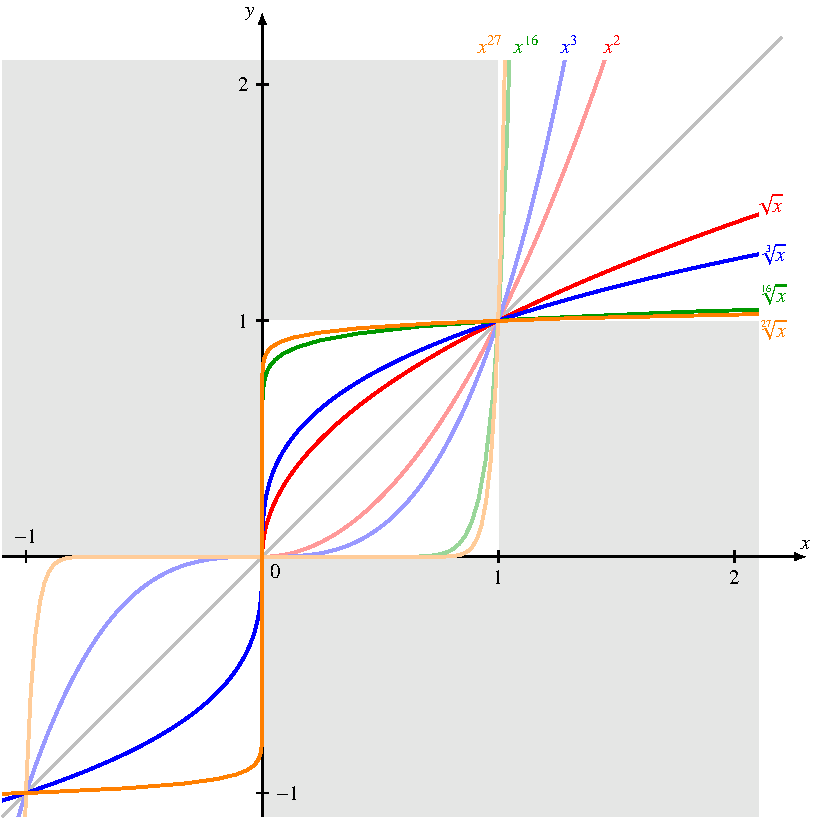
\includegraphics{chapters/010-potenzen/images/wurzel.pdf}
\caption[Graph der Wurzelfunktionen]{Graph der Wurzelfunktionen
%$x\mapsto\root{n}\of{x\mathstrut}$
\ensuremath{x\mapsto\root{n}\of{x}}
als Umkehrfunktionen der Potenzfunktionen $x\mapsto x^n$ für
$n=2$ ({\color{red}rot}), $n=3$ ({\color{blue}blau}),
$n=16$ ({\color{darkgreen}grün}) und $n=27$ ({\color{orange}orange}).
\label{buch:potenzen:fig:wurzel}
}
\end{figure}

\begin{definition}
Die inverse Funktion der Potenzfunktion
$f\colon \mathbb{R}\to\mathbb{R}:x\mapsto y=f(x)=x^n$
heisst die $n$-{\em te Wurzel} und wird
\[
\root{n}\of{\mathstrut\phantom{m}}
=
f^{-1}
\colon
D\to\mathbb{R}
:
y\mapsto f^{-1}(y)=\root{n}\of{\mathstrut y}
\]
geschrieben.
Für gerades $n$ ist der Definitionsbereich der Wurzel nur
$D=\mathbb{R}_{\ge 0}$, für ungerades $n$ ist $D=\mathbb{R}$.
Für $n=2$ wird die Wurzel als
\(
\root{2}\of{\mathstrut y}
=
\sqrt{\mathstrut y}
\)
geschrieben.
\end{definition}

TODO: Graph der Wurzelfunktion hinzufügen

Mit der Wurzelfunktion ist es jetzt möglich, auch kompliziertere
Gleichungen zu lösen:
\begin{enumerate}
\item
Für negative Argument $y<0$ müssen Quadratwurzeln als
$\sqrt{y\mathstrut}=i\sqrt{-y\mathstrut}$ definiert werden.
\item
Mindestens der Betrag der Wurzel einer komplexen Zahl lässt
sich jetzt sofort mittels $|\root{n}\of{c\mathstrut}|=\root{n}\of{|c|\mathstrut}$
berechnen.
Für das Argument sind jedoch die in
Abschnitt~\label{buch:geometrie:section:trigonometrisch} definierten
trigonometrischen Funktionen notwendig.
\item
Die quadratische Gleichung 
\[
ax^2+bx+c=0
\]
hat die Nullstellen
\[
x_{1,2} = \frac{-b\pm\sqrt{b^2-4ac\mathstrut}}{2a}.
\]
\item
Für kubische Gleichungen hat Cardano eine Lösung gefunden, die
Nur Wurzelausdrücke und arithmetische Operationen verwendet.
Die Gleichung $x^3+px+q=0$ hat die Nullstelle
\[
x
=
\root{3}\of{-\frac{q}2+\sqrt{\frac{q^2}4+\frac{p^3}{27}}}
+
\root{3}\of{-\frac{q}2-\sqrt{\frac{q^2}4+\frac{p^3}{27}}}.
\]
Falls das Argument der Quadratwurzel negativ ist, muss eine
Kubikwurzel aus einer komplexen Zahl berechnet werden, was
wieder über die Möglichkeiten der oben definierten Wurzelfunktionen
hinausgeht.
\item
Für die Lösung einer Gleichung vierten Grades hat Ferrari eine
Formel angegeben, die mit Wurzelausdrücken und arithmetischen
Operationen auskommt.
\end{enumerate}

Allerdings ist damit auch bereits ausgeschöpft, was die
Wurzelfunktionen zur Lösung von Polynomgleichungen beitragen
können.
Der folgende Satz von Abel zeigt, dass man für Polynomgleichungen
höheren Grades nicht mit einer Lösung durch Wurzelausdrücke
rechnen kann.

\begin{satz}[Abel]
Für Polynomegleichungen vom Grad $n\ge 5$ gibt es keine allgemeine
Lösung durch Wurzelausdrücke.
\end{satz}


\section{Tschebyscheff-Filter}

Als Einstieg betrachten wir das Tschebyscheff-Filter, welches sehr verwandt ist mit dem elliptischen Filter.
Genauer ausgedrückt erhält man die Tschebyscheff-1 und -2 Filter bei Grenzwerten von Parametern beim elliptischen Filter.
Der Name des Filters deutet schon an, dass die Tschebyscheff-Polynome $T_N$ (siehe auch Kapitel \ref{buch:polynome:section:tschebyscheff}) für das Filter relevant sind:
\begin{align}
    T_{0}(x)&=1\\
    T_{1}(x)&=x\\
    T_{2}(x)&=2x^{2}-1\\
    T_{3}(x)&=4x^{3}-3x\\
    T_{n+1}(x)&=2x~T_{n}(x)-T_{n-1}(x).
\end{align}
Bemerkenswert ist, dass die Polynome im Intervall $[-1, 1]$ mit der trigonometrischen Funktion
\begin{align} \label{ellfilter:eq:chebychef_polynomials}
    T_N(w) &= \cos \left( N \cos^{-1}(w) \right) \\
           &= \cos \left(N~z \right), \quad w= \cos(z)
\end{align}
übereinstimmen.
Der Zusammenhang lässt sich mit den Doppel- und Mehrfachwinkelfunktionen der trigonometrischen Funktionen erklären.
Abbildung \ref{ellfilter:fig:chebychef_polynomials} zeigt einige Tschebyscheff-Polynome, wobei das Equiripple-Verhalten schon sichtbar ist.
\begin{figure}
    \centering
    %% Creator: Matplotlib, PGF backend
%%
%% To include the figure in your LaTeX document, write
%%   \input{<filename>.pgf}
%%
%% Make sure the required packages are loaded in your preamble
%%   \usepackage{pgf}
%%
%% Also ensure that all the required font packages are loaded; for instance,
%% the lmodern package is sometimes necessary when using math font.
%%   \usepackage{lmodern}
%%
%% Figures using additional raster images can only be included by \input if
%% they are in the same directory as the main LaTeX file. For loading figures
%% from other directories you can use the `import` package
%%   \usepackage{import}
%%
%% and then include the figures with
%%   \import{<path to file>}{<filename>.pgf}
%%
%% Matplotlib used the following preamble
%%
\begingroup%
\makeatletter%
\begin{pgfpicture}%
\pgfpathrectangle{\pgfpointorigin}{\pgfqpoint{5.500000in}{2.500000in}}%
\pgfusepath{use as bounding box, clip}%
\begin{pgfscope}%
\pgfsetbuttcap%
\pgfsetmiterjoin%
\pgfsetlinewidth{0.000000pt}%
\definecolor{currentstroke}{rgb}{1.000000,1.000000,1.000000}%
\pgfsetstrokecolor{currentstroke}%
\pgfsetstrokeopacity{0.000000}%
\pgfsetdash{}{0pt}%
\pgfpathmoveto{\pgfqpoint{0.000000in}{0.000000in}}%
\pgfpathlineto{\pgfqpoint{5.500000in}{0.000000in}}%
\pgfpathlineto{\pgfqpoint{5.500000in}{2.500000in}}%
\pgfpathlineto{\pgfqpoint{0.000000in}{2.500000in}}%
\pgfpathlineto{\pgfqpoint{0.000000in}{0.000000in}}%
\pgfpathclose%
\pgfusepath{}%
\end{pgfscope}%
\begin{pgfscope}%
\pgfsetbuttcap%
\pgfsetmiterjoin%
\definecolor{currentfill}{rgb}{1.000000,1.000000,1.000000}%
\pgfsetfillcolor{currentfill}%
\pgfsetlinewidth{0.000000pt}%
\definecolor{currentstroke}{rgb}{0.000000,0.000000,0.000000}%
\pgfsetstrokecolor{currentstroke}%
\pgfsetstrokeopacity{0.000000}%
\pgfsetdash{}{0pt}%
\pgfpathmoveto{\pgfqpoint{0.617954in}{0.548769in}}%
\pgfpathlineto{\pgfqpoint{5.350000in}{0.548769in}}%
\pgfpathlineto{\pgfqpoint{5.350000in}{2.301955in}}%
\pgfpathlineto{\pgfqpoint{0.617954in}{2.301955in}}%
\pgfpathlineto{\pgfqpoint{0.617954in}{0.548769in}}%
\pgfpathclose%
\pgfusepath{fill}%
\end{pgfscope}%
\begin{pgfscope}%
\pgfpathrectangle{\pgfqpoint{0.617954in}{0.548769in}}{\pgfqpoint{4.732046in}{1.753186in}}%
\pgfusepath{clip}%
\pgfsetrectcap%
\pgfsetroundjoin%
\pgfsetlinewidth{0.803000pt}%
\definecolor{currentstroke}{rgb}{0.690196,0.690196,0.690196}%
\pgfsetstrokecolor{currentstroke}%
\pgfsetdash{}{0pt}%
\pgfpathmoveto{\pgfqpoint{1.012292in}{0.548769in}}%
\pgfpathlineto{\pgfqpoint{1.012292in}{2.301955in}}%
\pgfusepath{stroke}%
\end{pgfscope}%
\begin{pgfscope}%
\pgfsetbuttcap%
\pgfsetroundjoin%
\definecolor{currentfill}{rgb}{0.000000,0.000000,0.000000}%
\pgfsetfillcolor{currentfill}%
\pgfsetlinewidth{0.803000pt}%
\definecolor{currentstroke}{rgb}{0.000000,0.000000,0.000000}%
\pgfsetstrokecolor{currentstroke}%
\pgfsetdash{}{0pt}%
\pgfsys@defobject{currentmarker}{\pgfqpoint{0.000000in}{-0.048611in}}{\pgfqpoint{0.000000in}{0.000000in}}{%
\pgfpathmoveto{\pgfqpoint{0.000000in}{0.000000in}}%
\pgfpathlineto{\pgfqpoint{0.000000in}{-0.048611in}}%
\pgfusepath{stroke,fill}%
}%
\begin{pgfscope}%
\pgfsys@transformshift{1.012292in}{0.548769in}%
\pgfsys@useobject{currentmarker}{}%
\end{pgfscope}%
\end{pgfscope}%
\begin{pgfscope}%
\definecolor{textcolor}{rgb}{0.000000,0.000000,0.000000}%
\pgfsetstrokecolor{textcolor}%
\pgfsetfillcolor{textcolor}%
\pgftext[x=1.012292in,y=0.451547in,,top]{\color{textcolor}\rmfamily\fontsize{10.000000}{12.000000}\selectfont \(\displaystyle {\ensuremath{-}1.0}\)}%
\end{pgfscope}%
\begin{pgfscope}%
\pgfpathrectangle{\pgfqpoint{0.617954in}{0.548769in}}{\pgfqpoint{4.732046in}{1.753186in}}%
\pgfusepath{clip}%
\pgfsetrectcap%
\pgfsetroundjoin%
\pgfsetlinewidth{0.803000pt}%
\definecolor{currentstroke}{rgb}{0.690196,0.690196,0.690196}%
\pgfsetstrokecolor{currentstroke}%
\pgfsetdash{}{0pt}%
\pgfpathmoveto{\pgfqpoint{1.998134in}{0.548769in}}%
\pgfpathlineto{\pgfqpoint{1.998134in}{2.301955in}}%
\pgfusepath{stroke}%
\end{pgfscope}%
\begin{pgfscope}%
\pgfsetbuttcap%
\pgfsetroundjoin%
\definecolor{currentfill}{rgb}{0.000000,0.000000,0.000000}%
\pgfsetfillcolor{currentfill}%
\pgfsetlinewidth{0.803000pt}%
\definecolor{currentstroke}{rgb}{0.000000,0.000000,0.000000}%
\pgfsetstrokecolor{currentstroke}%
\pgfsetdash{}{0pt}%
\pgfsys@defobject{currentmarker}{\pgfqpoint{0.000000in}{-0.048611in}}{\pgfqpoint{0.000000in}{0.000000in}}{%
\pgfpathmoveto{\pgfqpoint{0.000000in}{0.000000in}}%
\pgfpathlineto{\pgfqpoint{0.000000in}{-0.048611in}}%
\pgfusepath{stroke,fill}%
}%
\begin{pgfscope}%
\pgfsys@transformshift{1.998134in}{0.548769in}%
\pgfsys@useobject{currentmarker}{}%
\end{pgfscope}%
\end{pgfscope}%
\begin{pgfscope}%
\definecolor{textcolor}{rgb}{0.000000,0.000000,0.000000}%
\pgfsetstrokecolor{textcolor}%
\pgfsetfillcolor{textcolor}%
\pgftext[x=1.998134in,y=0.451547in,,top]{\color{textcolor}\rmfamily\fontsize{10.000000}{12.000000}\selectfont \(\displaystyle {\ensuremath{-}0.5}\)}%
\end{pgfscope}%
\begin{pgfscope}%
\pgfpathrectangle{\pgfqpoint{0.617954in}{0.548769in}}{\pgfqpoint{4.732046in}{1.753186in}}%
\pgfusepath{clip}%
\pgfsetrectcap%
\pgfsetroundjoin%
\pgfsetlinewidth{0.803000pt}%
\definecolor{currentstroke}{rgb}{0.690196,0.690196,0.690196}%
\pgfsetstrokecolor{currentstroke}%
\pgfsetdash{}{0pt}%
\pgfpathmoveto{\pgfqpoint{2.983977in}{0.548769in}}%
\pgfpathlineto{\pgfqpoint{2.983977in}{2.301955in}}%
\pgfusepath{stroke}%
\end{pgfscope}%
\begin{pgfscope}%
\pgfsetbuttcap%
\pgfsetroundjoin%
\definecolor{currentfill}{rgb}{0.000000,0.000000,0.000000}%
\pgfsetfillcolor{currentfill}%
\pgfsetlinewidth{0.803000pt}%
\definecolor{currentstroke}{rgb}{0.000000,0.000000,0.000000}%
\pgfsetstrokecolor{currentstroke}%
\pgfsetdash{}{0pt}%
\pgfsys@defobject{currentmarker}{\pgfqpoint{0.000000in}{-0.048611in}}{\pgfqpoint{0.000000in}{0.000000in}}{%
\pgfpathmoveto{\pgfqpoint{0.000000in}{0.000000in}}%
\pgfpathlineto{\pgfqpoint{0.000000in}{-0.048611in}}%
\pgfusepath{stroke,fill}%
}%
\begin{pgfscope}%
\pgfsys@transformshift{2.983977in}{0.548769in}%
\pgfsys@useobject{currentmarker}{}%
\end{pgfscope}%
\end{pgfscope}%
\begin{pgfscope}%
\definecolor{textcolor}{rgb}{0.000000,0.000000,0.000000}%
\pgfsetstrokecolor{textcolor}%
\pgfsetfillcolor{textcolor}%
\pgftext[x=2.983977in,y=0.451547in,,top]{\color{textcolor}\rmfamily\fontsize{10.000000}{12.000000}\selectfont \(\displaystyle {0.0}\)}%
\end{pgfscope}%
\begin{pgfscope}%
\pgfpathrectangle{\pgfqpoint{0.617954in}{0.548769in}}{\pgfqpoint{4.732046in}{1.753186in}}%
\pgfusepath{clip}%
\pgfsetrectcap%
\pgfsetroundjoin%
\pgfsetlinewidth{0.803000pt}%
\definecolor{currentstroke}{rgb}{0.690196,0.690196,0.690196}%
\pgfsetstrokecolor{currentstroke}%
\pgfsetdash{}{0pt}%
\pgfpathmoveto{\pgfqpoint{3.969820in}{0.548769in}}%
\pgfpathlineto{\pgfqpoint{3.969820in}{2.301955in}}%
\pgfusepath{stroke}%
\end{pgfscope}%
\begin{pgfscope}%
\pgfsetbuttcap%
\pgfsetroundjoin%
\definecolor{currentfill}{rgb}{0.000000,0.000000,0.000000}%
\pgfsetfillcolor{currentfill}%
\pgfsetlinewidth{0.803000pt}%
\definecolor{currentstroke}{rgb}{0.000000,0.000000,0.000000}%
\pgfsetstrokecolor{currentstroke}%
\pgfsetdash{}{0pt}%
\pgfsys@defobject{currentmarker}{\pgfqpoint{0.000000in}{-0.048611in}}{\pgfqpoint{0.000000in}{0.000000in}}{%
\pgfpathmoveto{\pgfqpoint{0.000000in}{0.000000in}}%
\pgfpathlineto{\pgfqpoint{0.000000in}{-0.048611in}}%
\pgfusepath{stroke,fill}%
}%
\begin{pgfscope}%
\pgfsys@transformshift{3.969820in}{0.548769in}%
\pgfsys@useobject{currentmarker}{}%
\end{pgfscope}%
\end{pgfscope}%
\begin{pgfscope}%
\definecolor{textcolor}{rgb}{0.000000,0.000000,0.000000}%
\pgfsetstrokecolor{textcolor}%
\pgfsetfillcolor{textcolor}%
\pgftext[x=3.969820in,y=0.451547in,,top]{\color{textcolor}\rmfamily\fontsize{10.000000}{12.000000}\selectfont \(\displaystyle {0.5}\)}%
\end{pgfscope}%
\begin{pgfscope}%
\pgfpathrectangle{\pgfqpoint{0.617954in}{0.548769in}}{\pgfqpoint{4.732046in}{1.753186in}}%
\pgfusepath{clip}%
\pgfsetrectcap%
\pgfsetroundjoin%
\pgfsetlinewidth{0.803000pt}%
\definecolor{currentstroke}{rgb}{0.690196,0.690196,0.690196}%
\pgfsetstrokecolor{currentstroke}%
\pgfsetdash{}{0pt}%
\pgfpathmoveto{\pgfqpoint{4.955663in}{0.548769in}}%
\pgfpathlineto{\pgfqpoint{4.955663in}{2.301955in}}%
\pgfusepath{stroke}%
\end{pgfscope}%
\begin{pgfscope}%
\pgfsetbuttcap%
\pgfsetroundjoin%
\definecolor{currentfill}{rgb}{0.000000,0.000000,0.000000}%
\pgfsetfillcolor{currentfill}%
\pgfsetlinewidth{0.803000pt}%
\definecolor{currentstroke}{rgb}{0.000000,0.000000,0.000000}%
\pgfsetstrokecolor{currentstroke}%
\pgfsetdash{}{0pt}%
\pgfsys@defobject{currentmarker}{\pgfqpoint{0.000000in}{-0.048611in}}{\pgfqpoint{0.000000in}{0.000000in}}{%
\pgfpathmoveto{\pgfqpoint{0.000000in}{0.000000in}}%
\pgfpathlineto{\pgfqpoint{0.000000in}{-0.048611in}}%
\pgfusepath{stroke,fill}%
}%
\begin{pgfscope}%
\pgfsys@transformshift{4.955663in}{0.548769in}%
\pgfsys@useobject{currentmarker}{}%
\end{pgfscope}%
\end{pgfscope}%
\begin{pgfscope}%
\definecolor{textcolor}{rgb}{0.000000,0.000000,0.000000}%
\pgfsetstrokecolor{textcolor}%
\pgfsetfillcolor{textcolor}%
\pgftext[x=4.955663in,y=0.451547in,,top]{\color{textcolor}\rmfamily\fontsize{10.000000}{12.000000}\selectfont \(\displaystyle {1.0}\)}%
\end{pgfscope}%
\begin{pgfscope}%
\definecolor{textcolor}{rgb}{0.000000,0.000000,0.000000}%
\pgfsetstrokecolor{textcolor}%
\pgfsetfillcolor{textcolor}%
\pgftext[x=2.983977in,y=0.272534in,,top]{\color{textcolor}\rmfamily\fontsize{10.000000}{12.000000}\selectfont \(\displaystyle w\)}%
\end{pgfscope}%
\begin{pgfscope}%
\pgfpathrectangle{\pgfqpoint{0.617954in}{0.548769in}}{\pgfqpoint{4.732046in}{1.753186in}}%
\pgfusepath{clip}%
\pgfsetrectcap%
\pgfsetroundjoin%
\pgfsetlinewidth{0.803000pt}%
\definecolor{currentstroke}{rgb}{0.690196,0.690196,0.690196}%
\pgfsetstrokecolor{currentstroke}%
\pgfsetdash{}{0pt}%
\pgfpathmoveto{\pgfqpoint{0.617954in}{0.548769in}}%
\pgfpathlineto{\pgfqpoint{5.350000in}{0.548769in}}%
\pgfusepath{stroke}%
\end{pgfscope}%
\begin{pgfscope}%
\pgfsetbuttcap%
\pgfsetroundjoin%
\definecolor{currentfill}{rgb}{0.000000,0.000000,0.000000}%
\pgfsetfillcolor{currentfill}%
\pgfsetlinewidth{0.803000pt}%
\definecolor{currentstroke}{rgb}{0.000000,0.000000,0.000000}%
\pgfsetstrokecolor{currentstroke}%
\pgfsetdash{}{0pt}%
\pgfsys@defobject{currentmarker}{\pgfqpoint{-0.048611in}{0.000000in}}{\pgfqpoint{-0.000000in}{0.000000in}}{%
\pgfpathmoveto{\pgfqpoint{-0.000000in}{0.000000in}}%
\pgfpathlineto{\pgfqpoint{-0.048611in}{0.000000in}}%
\pgfusepath{stroke,fill}%
}%
\begin{pgfscope}%
\pgfsys@transformshift{0.617954in}{0.548769in}%
\pgfsys@useobject{currentmarker}{}%
\end{pgfscope}%
\end{pgfscope}%
\begin{pgfscope}%
\definecolor{textcolor}{rgb}{0.000000,0.000000,0.000000}%
\pgfsetstrokecolor{textcolor}%
\pgfsetfillcolor{textcolor}%
\pgftext[x=0.343262in, y=0.500544in, left, base]{\color{textcolor}\rmfamily\fontsize{10.000000}{12.000000}\selectfont \(\displaystyle {\ensuremath{-}2}\)}%
\end{pgfscope}%
\begin{pgfscope}%
\pgfpathrectangle{\pgfqpoint{0.617954in}{0.548769in}}{\pgfqpoint{4.732046in}{1.753186in}}%
\pgfusepath{clip}%
\pgfsetrectcap%
\pgfsetroundjoin%
\pgfsetlinewidth{0.803000pt}%
\definecolor{currentstroke}{rgb}{0.690196,0.690196,0.690196}%
\pgfsetstrokecolor{currentstroke}%
\pgfsetdash{}{0pt}%
\pgfpathmoveto{\pgfqpoint{0.617954in}{0.987065in}}%
\pgfpathlineto{\pgfqpoint{5.350000in}{0.987065in}}%
\pgfusepath{stroke}%
\end{pgfscope}%
\begin{pgfscope}%
\pgfsetbuttcap%
\pgfsetroundjoin%
\definecolor{currentfill}{rgb}{0.000000,0.000000,0.000000}%
\pgfsetfillcolor{currentfill}%
\pgfsetlinewidth{0.803000pt}%
\definecolor{currentstroke}{rgb}{0.000000,0.000000,0.000000}%
\pgfsetstrokecolor{currentstroke}%
\pgfsetdash{}{0pt}%
\pgfsys@defobject{currentmarker}{\pgfqpoint{-0.048611in}{0.000000in}}{\pgfqpoint{-0.000000in}{0.000000in}}{%
\pgfpathmoveto{\pgfqpoint{-0.000000in}{0.000000in}}%
\pgfpathlineto{\pgfqpoint{-0.048611in}{0.000000in}}%
\pgfusepath{stroke,fill}%
}%
\begin{pgfscope}%
\pgfsys@transformshift{0.617954in}{0.987065in}%
\pgfsys@useobject{currentmarker}{}%
\end{pgfscope}%
\end{pgfscope}%
\begin{pgfscope}%
\definecolor{textcolor}{rgb}{0.000000,0.000000,0.000000}%
\pgfsetstrokecolor{textcolor}%
\pgfsetfillcolor{textcolor}%
\pgftext[x=0.343262in, y=0.938840in, left, base]{\color{textcolor}\rmfamily\fontsize{10.000000}{12.000000}\selectfont \(\displaystyle {\ensuremath{-}1}\)}%
\end{pgfscope}%
\begin{pgfscope}%
\pgfpathrectangle{\pgfqpoint{0.617954in}{0.548769in}}{\pgfqpoint{4.732046in}{1.753186in}}%
\pgfusepath{clip}%
\pgfsetrectcap%
\pgfsetroundjoin%
\pgfsetlinewidth{0.803000pt}%
\definecolor{currentstroke}{rgb}{0.690196,0.690196,0.690196}%
\pgfsetstrokecolor{currentstroke}%
\pgfsetdash{}{0pt}%
\pgfpathmoveto{\pgfqpoint{0.617954in}{1.425362in}}%
\pgfpathlineto{\pgfqpoint{5.350000in}{1.425362in}}%
\pgfusepath{stroke}%
\end{pgfscope}%
\begin{pgfscope}%
\pgfsetbuttcap%
\pgfsetroundjoin%
\definecolor{currentfill}{rgb}{0.000000,0.000000,0.000000}%
\pgfsetfillcolor{currentfill}%
\pgfsetlinewidth{0.803000pt}%
\definecolor{currentstroke}{rgb}{0.000000,0.000000,0.000000}%
\pgfsetstrokecolor{currentstroke}%
\pgfsetdash{}{0pt}%
\pgfsys@defobject{currentmarker}{\pgfqpoint{-0.048611in}{0.000000in}}{\pgfqpoint{-0.000000in}{0.000000in}}{%
\pgfpathmoveto{\pgfqpoint{-0.000000in}{0.000000in}}%
\pgfpathlineto{\pgfqpoint{-0.048611in}{0.000000in}}%
\pgfusepath{stroke,fill}%
}%
\begin{pgfscope}%
\pgfsys@transformshift{0.617954in}{1.425362in}%
\pgfsys@useobject{currentmarker}{}%
\end{pgfscope}%
\end{pgfscope}%
\begin{pgfscope}%
\definecolor{textcolor}{rgb}{0.000000,0.000000,0.000000}%
\pgfsetstrokecolor{textcolor}%
\pgfsetfillcolor{textcolor}%
\pgftext[x=0.451287in, y=1.377137in, left, base]{\color{textcolor}\rmfamily\fontsize{10.000000}{12.000000}\selectfont \(\displaystyle {0}\)}%
\end{pgfscope}%
\begin{pgfscope}%
\pgfpathrectangle{\pgfqpoint{0.617954in}{0.548769in}}{\pgfqpoint{4.732046in}{1.753186in}}%
\pgfusepath{clip}%
\pgfsetrectcap%
\pgfsetroundjoin%
\pgfsetlinewidth{0.803000pt}%
\definecolor{currentstroke}{rgb}{0.690196,0.690196,0.690196}%
\pgfsetstrokecolor{currentstroke}%
\pgfsetdash{}{0pt}%
\pgfpathmoveto{\pgfqpoint{0.617954in}{1.863658in}}%
\pgfpathlineto{\pgfqpoint{5.350000in}{1.863658in}}%
\pgfusepath{stroke}%
\end{pgfscope}%
\begin{pgfscope}%
\pgfsetbuttcap%
\pgfsetroundjoin%
\definecolor{currentfill}{rgb}{0.000000,0.000000,0.000000}%
\pgfsetfillcolor{currentfill}%
\pgfsetlinewidth{0.803000pt}%
\definecolor{currentstroke}{rgb}{0.000000,0.000000,0.000000}%
\pgfsetstrokecolor{currentstroke}%
\pgfsetdash{}{0pt}%
\pgfsys@defobject{currentmarker}{\pgfqpoint{-0.048611in}{0.000000in}}{\pgfqpoint{-0.000000in}{0.000000in}}{%
\pgfpathmoveto{\pgfqpoint{-0.000000in}{0.000000in}}%
\pgfpathlineto{\pgfqpoint{-0.048611in}{0.000000in}}%
\pgfusepath{stroke,fill}%
}%
\begin{pgfscope}%
\pgfsys@transformshift{0.617954in}{1.863658in}%
\pgfsys@useobject{currentmarker}{}%
\end{pgfscope}%
\end{pgfscope}%
\begin{pgfscope}%
\definecolor{textcolor}{rgb}{0.000000,0.000000,0.000000}%
\pgfsetstrokecolor{textcolor}%
\pgfsetfillcolor{textcolor}%
\pgftext[x=0.451287in, y=1.815433in, left, base]{\color{textcolor}\rmfamily\fontsize{10.000000}{12.000000}\selectfont \(\displaystyle {1}\)}%
\end{pgfscope}%
\begin{pgfscope}%
\pgfpathrectangle{\pgfqpoint{0.617954in}{0.548769in}}{\pgfqpoint{4.732046in}{1.753186in}}%
\pgfusepath{clip}%
\pgfsetrectcap%
\pgfsetroundjoin%
\pgfsetlinewidth{0.803000pt}%
\definecolor{currentstroke}{rgb}{0.690196,0.690196,0.690196}%
\pgfsetstrokecolor{currentstroke}%
\pgfsetdash{}{0pt}%
\pgfpathmoveto{\pgfqpoint{0.617954in}{2.301955in}}%
\pgfpathlineto{\pgfqpoint{5.350000in}{2.301955in}}%
\pgfusepath{stroke}%
\end{pgfscope}%
\begin{pgfscope}%
\pgfsetbuttcap%
\pgfsetroundjoin%
\definecolor{currentfill}{rgb}{0.000000,0.000000,0.000000}%
\pgfsetfillcolor{currentfill}%
\pgfsetlinewidth{0.803000pt}%
\definecolor{currentstroke}{rgb}{0.000000,0.000000,0.000000}%
\pgfsetstrokecolor{currentstroke}%
\pgfsetdash{}{0pt}%
\pgfsys@defobject{currentmarker}{\pgfqpoint{-0.048611in}{0.000000in}}{\pgfqpoint{-0.000000in}{0.000000in}}{%
\pgfpathmoveto{\pgfqpoint{-0.000000in}{0.000000in}}%
\pgfpathlineto{\pgfqpoint{-0.048611in}{0.000000in}}%
\pgfusepath{stroke,fill}%
}%
\begin{pgfscope}%
\pgfsys@transformshift{0.617954in}{2.301955in}%
\pgfsys@useobject{currentmarker}{}%
\end{pgfscope}%
\end{pgfscope}%
\begin{pgfscope}%
\definecolor{textcolor}{rgb}{0.000000,0.000000,0.000000}%
\pgfsetstrokecolor{textcolor}%
\pgfsetfillcolor{textcolor}%
\pgftext[x=0.451287in, y=2.253730in, left, base]{\color{textcolor}\rmfamily\fontsize{10.000000}{12.000000}\selectfont \(\displaystyle {2}\)}%
\end{pgfscope}%
\begin{pgfscope}%
\definecolor{textcolor}{rgb}{0.000000,0.000000,0.000000}%
\pgfsetstrokecolor{textcolor}%
\pgfsetfillcolor{textcolor}%
\pgftext[x=0.287707in,y=1.425362in,,bottom,rotate=90.000000]{\color{textcolor}\rmfamily\fontsize{10.000000}{12.000000}\selectfont \(\displaystyle T_N(w)\)}%
\end{pgfscope}%
\begin{pgfscope}%
\pgfpathrectangle{\pgfqpoint{0.617954in}{0.548769in}}{\pgfqpoint{4.732046in}{1.753186in}}%
\pgfusepath{clip}%
\pgfsetrectcap%
\pgfsetroundjoin%
\pgfsetlinewidth{1.505625pt}%
\definecolor{currentstroke}{rgb}{0.121569,0.466667,0.705882}%
\pgfsetstrokecolor{currentstroke}%
\pgfsetdash{}{0pt}%
\pgfpathmoveto{\pgfqpoint{0.815123in}{0.538250in}}%
\pgfpathlineto{\pgfqpoint{0.867228in}{0.667673in}}%
\pgfpathlineto{\pgfqpoint{0.919332in}{0.789210in}}%
\pgfpathlineto{\pgfqpoint{0.971437in}{0.903055in}}%
\pgfpathlineto{\pgfqpoint{1.023541in}{1.009402in}}%
\pgfpathlineto{\pgfqpoint{1.075646in}{1.108444in}}%
\pgfpathlineto{\pgfqpoint{1.123409in}{1.192982in}}%
\pgfpathlineto{\pgfqpoint{1.171171in}{1.271695in}}%
\pgfpathlineto{\pgfqpoint{1.218934in}{1.344733in}}%
\pgfpathlineto{\pgfqpoint{1.266696in}{1.412244in}}%
\pgfpathlineto{\pgfqpoint{1.314459in}{1.474380in}}%
\pgfpathlineto{\pgfqpoint{1.362221in}{1.531289in}}%
\pgfpathlineto{\pgfqpoint{1.409984in}{1.583121in}}%
\pgfpathlineto{\pgfqpoint{1.453404in}{1.625960in}}%
\pgfpathlineto{\pgfqpoint{1.496825in}{1.664840in}}%
\pgfpathlineto{\pgfqpoint{1.540245in}{1.699871in}}%
\pgfpathlineto{\pgfqpoint{1.583666in}{1.731168in}}%
\pgfpathlineto{\pgfqpoint{1.627086in}{1.758841in}}%
\pgfpathlineto{\pgfqpoint{1.670507in}{1.783003in}}%
\pgfpathlineto{\pgfqpoint{1.713927in}{1.803767in}}%
\pgfpathlineto{\pgfqpoint{1.757348in}{1.821245in}}%
\pgfpathlineto{\pgfqpoint{1.800768in}{1.835549in}}%
\pgfpathlineto{\pgfqpoint{1.844189in}{1.846792in}}%
\pgfpathlineto{\pgfqpoint{1.887609in}{1.855086in}}%
\pgfpathlineto{\pgfqpoint{1.935372in}{1.860937in}}%
\pgfpathlineto{\pgfqpoint{1.983135in}{1.863505in}}%
\pgfpathlineto{\pgfqpoint{2.030897in}{1.862940in}}%
\pgfpathlineto{\pgfqpoint{2.078660in}{1.859391in}}%
\pgfpathlineto{\pgfqpoint{2.130764in}{1.852293in}}%
\pgfpathlineto{\pgfqpoint{2.182869in}{1.842015in}}%
\pgfpathlineto{\pgfqpoint{2.239316in}{1.827518in}}%
\pgfpathlineto{\pgfqpoint{2.295762in}{1.809766in}}%
\pgfpathlineto{\pgfqpoint{2.356551in}{1.787290in}}%
\pgfpathlineto{\pgfqpoint{2.421682in}{1.759685in}}%
\pgfpathlineto{\pgfqpoint{2.491154in}{1.726641in}}%
\pgfpathlineto{\pgfqpoint{2.564969in}{1.687966in}}%
\pgfpathlineto{\pgfqpoint{2.647468in}{1.641059in}}%
\pgfpathlineto{\pgfqpoint{2.738651in}{1.585589in}}%
\pgfpathlineto{\pgfqpoint{2.851545in}{1.513148in}}%
\pgfpathlineto{\pgfqpoint{3.064305in}{1.371911in}}%
\pgfpathlineto{\pgfqpoint{3.207593in}{1.278793in}}%
\pgfpathlineto{\pgfqpoint{3.307460in}{1.217378in}}%
\pgfpathlineto{\pgfqpoint{3.394301in}{1.167524in}}%
\pgfpathlineto{\pgfqpoint{3.472458in}{1.126261in}}%
\pgfpathlineto{\pgfqpoint{3.541931in}{1.093000in}}%
\pgfpathlineto{\pgfqpoint{3.607061in}{1.065165in}}%
\pgfpathlineto{\pgfqpoint{3.667850in}{1.042451in}}%
\pgfpathlineto{\pgfqpoint{3.724297in}{1.024458in}}%
\pgfpathlineto{\pgfqpoint{3.780743in}{1.009703in}}%
\pgfpathlineto{\pgfqpoint{3.832848in}{0.999169in}}%
\pgfpathlineto{\pgfqpoint{3.884953in}{0.991798in}}%
\pgfpathlineto{\pgfqpoint{3.932715in}{0.987985in}}%
\pgfpathlineto{\pgfqpoint{3.980478in}{0.987142in}}%
\pgfpathlineto{\pgfqpoint{4.028240in}{0.989420in}}%
\pgfpathlineto{\pgfqpoint{4.076003in}{0.994966in}}%
\pgfpathlineto{\pgfqpoint{4.119423in}{1.002971in}}%
\pgfpathlineto{\pgfqpoint{4.162844in}{1.013914in}}%
\pgfpathlineto{\pgfqpoint{4.206264in}{1.027907in}}%
\pgfpathlineto{\pgfqpoint{4.249685in}{1.045063in}}%
\pgfpathlineto{\pgfqpoint{4.293105in}{1.065493in}}%
\pgfpathlineto{\pgfqpoint{4.336526in}{1.089310in}}%
\pgfpathlineto{\pgfqpoint{4.379946in}{1.116627in}}%
\pgfpathlineto{\pgfqpoint{4.423367in}{1.147556in}}%
\pgfpathlineto{\pgfqpoint{4.466787in}{1.182209in}}%
\pgfpathlineto{\pgfqpoint{4.510208in}{1.220699in}}%
\pgfpathlineto{\pgfqpoint{4.553628in}{1.263138in}}%
\pgfpathlineto{\pgfqpoint{4.597049in}{1.309638in}}%
\pgfpathlineto{\pgfqpoint{4.644812in}{1.365612in}}%
\pgfpathlineto{\pgfqpoint{4.692574in}{1.426786in}}%
\pgfpathlineto{\pgfqpoint{4.740337in}{1.493310in}}%
\pgfpathlineto{\pgfqpoint{4.788099in}{1.565332in}}%
\pgfpathlineto{\pgfqpoint{4.835862in}{1.643002in}}%
\pgfpathlineto{\pgfqpoint{4.883624in}{1.726469in}}%
\pgfpathlineto{\pgfqpoint{4.931387in}{1.815884in}}%
\pgfpathlineto{\pgfqpoint{4.983491in}{1.920387in}}%
\pgfpathlineto{\pgfqpoint{5.035596in}{2.032338in}}%
\pgfpathlineto{\pgfqpoint{5.087701in}{2.151934in}}%
\pgfpathlineto{\pgfqpoint{5.139805in}{2.279368in}}%
\pgfpathlineto{\pgfqpoint{5.152831in}{2.312474in}}%
\pgfpathlineto{\pgfqpoint{5.152831in}{2.312474in}}%
\pgfusepath{stroke}%
\end{pgfscope}%
\begin{pgfscope}%
\pgfpathrectangle{\pgfqpoint{0.617954in}{0.548769in}}{\pgfqpoint{4.732046in}{1.753186in}}%
\pgfusepath{clip}%
\pgfsetrectcap%
\pgfsetroundjoin%
\pgfsetlinewidth{1.505625pt}%
\definecolor{currentstroke}{rgb}{1.000000,0.498039,0.054902}%
\pgfsetstrokecolor{currentstroke}%
\pgfsetdash{}{0pt}%
\pgfpathmoveto{\pgfqpoint{0.963285in}{2.315844in}}%
\pgfpathlineto{\pgfqpoint{0.988805in}{2.065008in}}%
\pgfpathlineto{\pgfqpoint{1.014857in}{1.843281in}}%
\pgfpathlineto{\pgfqpoint{1.036568in}{1.682977in}}%
\pgfpathlineto{\pgfqpoint{1.058278in}{1.543280in}}%
\pgfpathlineto{\pgfqpoint{1.079988in}{1.422723in}}%
\pgfpathlineto{\pgfqpoint{1.101698in}{1.319903in}}%
\pgfpathlineto{\pgfqpoint{1.123409in}{1.233476in}}%
\pgfpathlineto{\pgfqpoint{1.140777in}{1.175276in}}%
\pgfpathlineto{\pgfqpoint{1.158145in}{1.126117in}}%
\pgfpathlineto{\pgfqpoint{1.175513in}{1.085395in}}%
\pgfpathlineto{\pgfqpoint{1.192881in}{1.052526in}}%
\pgfpathlineto{\pgfqpoint{1.210250in}{1.026952in}}%
\pgfpathlineto{\pgfqpoint{1.223276in}{1.012233in}}%
\pgfpathlineto{\pgfqpoint{1.236302in}{1.001095in}}%
\pgfpathlineto{\pgfqpoint{1.249328in}{0.993325in}}%
\pgfpathlineto{\pgfqpoint{1.262354in}{0.988718in}}%
\pgfpathlineto{\pgfqpoint{1.275380in}{0.987075in}}%
\pgfpathlineto{\pgfqpoint{1.288407in}{0.988202in}}%
\pgfpathlineto{\pgfqpoint{1.301433in}{0.991914in}}%
\pgfpathlineto{\pgfqpoint{1.318801in}{1.000572in}}%
\pgfpathlineto{\pgfqpoint{1.336169in}{1.013093in}}%
\pgfpathlineto{\pgfqpoint{1.353537in}{1.029086in}}%
\pgfpathlineto{\pgfqpoint{1.375248in}{1.053389in}}%
\pgfpathlineto{\pgfqpoint{1.401300in}{1.087971in}}%
\pgfpathlineto{\pgfqpoint{1.431694in}{1.134386in}}%
\pgfpathlineto{\pgfqpoint{1.466431in}{1.193454in}}%
\pgfpathlineto{\pgfqpoint{1.514193in}{1.281335in}}%
\pgfpathlineto{\pgfqpoint{1.648797in}{1.533319in}}%
\pgfpathlineto{\pgfqpoint{1.692217in}{1.606504in}}%
\pgfpathlineto{\pgfqpoint{1.731296in}{1.666194in}}%
\pgfpathlineto{\pgfqpoint{1.766032in}{1.713499in}}%
\pgfpathlineto{\pgfqpoint{1.796426in}{1.750004in}}%
\pgfpathlineto{\pgfqpoint{1.826821in}{1.781659in}}%
\pgfpathlineto{\pgfqpoint{1.852873in}{1.804782in}}%
\pgfpathlineto{\pgfqpoint{1.878925in}{1.824113in}}%
\pgfpathlineto{\pgfqpoint{1.904978in}{1.839604in}}%
\pgfpathlineto{\pgfqpoint{1.931030in}{1.851242in}}%
\pgfpathlineto{\pgfqpoint{1.957082in}{1.859041in}}%
\pgfpathlineto{\pgfqpoint{1.983135in}{1.863047in}}%
\pgfpathlineto{\pgfqpoint{2.009187in}{1.863329in}}%
\pgfpathlineto{\pgfqpoint{2.035239in}{1.859984in}}%
\pgfpathlineto{\pgfqpoint{2.061291in}{1.853128in}}%
\pgfpathlineto{\pgfqpoint{2.087344in}{1.842898in}}%
\pgfpathlineto{\pgfqpoint{2.113396in}{1.829452in}}%
\pgfpathlineto{\pgfqpoint{2.143790in}{1.809929in}}%
\pgfpathlineto{\pgfqpoint{2.174185in}{1.786560in}}%
\pgfpathlineto{\pgfqpoint{2.208921in}{1.755558in}}%
\pgfpathlineto{\pgfqpoint{2.243658in}{1.720467in}}%
\pgfpathlineto{\pgfqpoint{2.282736in}{1.676770in}}%
\pgfpathlineto{\pgfqpoint{2.330499in}{1.618420in}}%
\pgfpathlineto{\pgfqpoint{2.386945in}{1.544378in}}%
\pgfpathlineto{\pgfqpoint{2.491154in}{1.401257in}}%
\pgfpathlineto{\pgfqpoint{2.573653in}{1.290423in}}%
\pgfpathlineto{\pgfqpoint{2.630100in}{1.219842in}}%
\pgfpathlineto{\pgfqpoint{2.677863in}{1.165204in}}%
\pgfpathlineto{\pgfqpoint{2.716941in}{1.124786in}}%
\pgfpathlineto{\pgfqpoint{2.756020in}{1.088796in}}%
\pgfpathlineto{\pgfqpoint{2.790756in}{1.060903in}}%
\pgfpathlineto{\pgfqpoint{2.825492in}{1.037164in}}%
\pgfpathlineto{\pgfqpoint{2.855887in}{1.019988in}}%
\pgfpathlineto{\pgfqpoint{2.886281in}{1.006308in}}%
\pgfpathlineto{\pgfqpoint{2.916675in}{0.996229in}}%
\pgfpathlineto{\pgfqpoint{2.947070in}{0.989827in}}%
\pgfpathlineto{\pgfqpoint{2.973122in}{0.987304in}}%
\pgfpathlineto{\pgfqpoint{2.999174in}{0.987534in}}%
\pgfpathlineto{\pgfqpoint{3.025227in}{0.990514in}}%
\pgfpathlineto{\pgfqpoint{3.051279in}{0.996229in}}%
\pgfpathlineto{\pgfqpoint{3.081673in}{1.006308in}}%
\pgfpathlineto{\pgfqpoint{3.112068in}{1.019988in}}%
\pgfpathlineto{\pgfqpoint{3.142462in}{1.037164in}}%
\pgfpathlineto{\pgfqpoint{3.172856in}{1.057704in}}%
\pgfpathlineto{\pgfqpoint{3.207593in}{1.085092in}}%
\pgfpathlineto{\pgfqpoint{3.242329in}{1.116388in}}%
\pgfpathlineto{\pgfqpoint{3.281408in}{1.155866in}}%
\pgfpathlineto{\pgfqpoint{3.324828in}{1.204423in}}%
\pgfpathlineto{\pgfqpoint{3.372591in}{1.262618in}}%
\pgfpathlineto{\pgfqpoint{3.433379in}{1.342111in}}%
\pgfpathlineto{\pgfqpoint{3.533247in}{1.479174in}}%
\pgfpathlineto{\pgfqpoint{3.615746in}{1.590473in}}%
\pgfpathlineto{\pgfqpoint{3.667850in}{1.656113in}}%
\pgfpathlineto{\pgfqpoint{3.711271in}{1.706362in}}%
\pgfpathlineto{\pgfqpoint{3.750349in}{1.747148in}}%
\pgfpathlineto{\pgfqpoint{3.785086in}{1.779222in}}%
\pgfpathlineto{\pgfqpoint{3.815480in}{1.803631in}}%
\pgfpathlineto{\pgfqpoint{3.845874in}{1.824284in}}%
\pgfpathlineto{\pgfqpoint{3.876269in}{1.840876in}}%
\pgfpathlineto{\pgfqpoint{3.902321in}{1.851653in}}%
\pgfpathlineto{\pgfqpoint{3.928373in}{1.859081in}}%
\pgfpathlineto{\pgfqpoint{3.954425in}{1.863021in}}%
\pgfpathlineto{\pgfqpoint{3.980478in}{1.863350in}}%
\pgfpathlineto{\pgfqpoint{4.002188in}{1.860795in}}%
\pgfpathlineto{\pgfqpoint{4.023898in}{1.855619in}}%
\pgfpathlineto{\pgfqpoint{4.049951in}{1.845904in}}%
\pgfpathlineto{\pgfqpoint{4.076003in}{1.832340in}}%
\pgfpathlineto{\pgfqpoint{4.102055in}{1.814925in}}%
\pgfpathlineto{\pgfqpoint{4.128108in}{1.793690in}}%
\pgfpathlineto{\pgfqpoint{4.154160in}{1.768700in}}%
\pgfpathlineto{\pgfqpoint{4.184554in}{1.734938in}}%
\pgfpathlineto{\pgfqpoint{4.214949in}{1.696434in}}%
\pgfpathlineto{\pgfqpoint{4.249685in}{1.647018in}}%
\pgfpathlineto{\pgfqpoint{4.288763in}{1.585242in}}%
\pgfpathlineto{\pgfqpoint{4.332184in}{1.510192in}}%
\pgfpathlineto{\pgfqpoint{4.388631in}{1.405562in}}%
\pgfpathlineto{\pgfqpoint{4.505866in}{1.185791in}}%
\pgfpathlineto{\pgfqpoint{4.544944in}{1.120547in}}%
\pgfpathlineto{\pgfqpoint{4.575339in}{1.075851in}}%
\pgfpathlineto{\pgfqpoint{4.601391in}{1.043132in}}%
\pgfpathlineto{\pgfqpoint{4.623101in}{1.020680in}}%
\pgfpathlineto{\pgfqpoint{4.640469in}{1.006375in}}%
\pgfpathlineto{\pgfqpoint{4.657838in}{0.995735in}}%
\pgfpathlineto{\pgfqpoint{4.675206in}{0.989161in}}%
\pgfpathlineto{\pgfqpoint{4.688232in}{0.987152in}}%
\pgfpathlineto{\pgfqpoint{4.701258in}{0.987850in}}%
\pgfpathlineto{\pgfqpoint{4.714284in}{0.991448in}}%
\pgfpathlineto{\pgfqpoint{4.727310in}{0.998141in}}%
\pgfpathlineto{\pgfqpoint{4.740337in}{1.008133in}}%
\pgfpathlineto{\pgfqpoint{4.753363in}{1.021634in}}%
\pgfpathlineto{\pgfqpoint{4.766389in}{1.038861in}}%
\pgfpathlineto{\pgfqpoint{4.783757in}{1.068014in}}%
\pgfpathlineto{\pgfqpoint{4.801125in}{1.104738in}}%
\pgfpathlineto{\pgfqpoint{4.818494in}{1.149605in}}%
\pgfpathlineto{\pgfqpoint{4.835862in}{1.203207in}}%
\pgfpathlineto{\pgfqpoint{4.853230in}{1.266163in}}%
\pgfpathlineto{\pgfqpoint{4.870598in}{1.339113in}}%
\pgfpathlineto{\pgfqpoint{4.892308in}{1.445372in}}%
\pgfpathlineto{\pgfqpoint{4.914019in}{1.569642in}}%
\pgfpathlineto{\pgfqpoint{4.935729in}{1.713341in}}%
\pgfpathlineto{\pgfqpoint{4.957439in}{1.877948in}}%
\pgfpathlineto{\pgfqpoint{4.979149in}{2.065008in}}%
\pgfpathlineto{\pgfqpoint{5.004669in}{2.315844in}}%
\pgfpathlineto{\pgfqpoint{5.004669in}{2.315844in}}%
\pgfusepath{stroke}%
\end{pgfscope}%
\begin{pgfscope}%
\pgfpathrectangle{\pgfqpoint{0.617954in}{0.548769in}}{\pgfqpoint{4.732046in}{1.753186in}}%
\pgfusepath{clip}%
\pgfsetrectcap%
\pgfsetroundjoin%
\pgfsetlinewidth{1.505625pt}%
\definecolor{currentstroke}{rgb}{0.172549,0.627451,0.172549}%
\pgfsetstrokecolor{currentstroke}%
\pgfsetdash{}{0pt}%
\pgfpathmoveto{\pgfqpoint{0.997762in}{0.534880in}}%
\pgfpathlineto{\pgfqpoint{1.010515in}{0.938420in}}%
\pgfpathlineto{\pgfqpoint{1.023541in}{1.256633in}}%
\pgfpathlineto{\pgfqpoint{1.036568in}{1.493946in}}%
\pgfpathlineto{\pgfqpoint{1.049594in}{1.662731in}}%
\pgfpathlineto{\pgfqpoint{1.058278in}{1.742696in}}%
\pgfpathlineto{\pgfqpoint{1.066962in}{1.800120in}}%
\pgfpathlineto{\pgfqpoint{1.075646in}{1.837754in}}%
\pgfpathlineto{\pgfqpoint{1.084330in}{1.858134in}}%
\pgfpathlineto{\pgfqpoint{1.088672in}{1.862591in}}%
\pgfpathlineto{\pgfqpoint{1.093014in}{1.863596in}}%
\pgfpathlineto{\pgfqpoint{1.097356in}{1.861410in}}%
\pgfpathlineto{\pgfqpoint{1.101698in}{1.856284in}}%
\pgfpathlineto{\pgfqpoint{1.110382in}{1.838165in}}%
\pgfpathlineto{\pgfqpoint{1.119067in}{1.811034in}}%
\pgfpathlineto{\pgfqpoint{1.132093in}{1.756980in}}%
\pgfpathlineto{\pgfqpoint{1.149461in}{1.667415in}}%
\pgfpathlineto{\pgfqpoint{1.179855in}{1.488530in}}%
\pgfpathlineto{\pgfqpoint{1.214592in}{1.289910in}}%
\pgfpathlineto{\pgfqpoint{1.236302in}{1.184400in}}%
\pgfpathlineto{\pgfqpoint{1.253670in}{1.114719in}}%
\pgfpathlineto{\pgfqpoint{1.266696in}{1.072074in}}%
\pgfpathlineto{\pgfqpoint{1.279722in}{1.038054in}}%
\pgfpathlineto{\pgfqpoint{1.292749in}{1.012779in}}%
\pgfpathlineto{\pgfqpoint{1.301433in}{1.000762in}}%
\pgfpathlineto{\pgfqpoint{1.310117in}{0.992549in}}%
\pgfpathlineto{\pgfqpoint{1.318801in}{0.988057in}}%
\pgfpathlineto{\pgfqpoint{1.327485in}{0.987177in}}%
\pgfpathlineto{\pgfqpoint{1.336169in}{0.989782in}}%
\pgfpathlineto{\pgfqpoint{1.344853in}{0.995723in}}%
\pgfpathlineto{\pgfqpoint{1.353537in}{1.004838in}}%
\pgfpathlineto{\pgfqpoint{1.366563in}{1.024074in}}%
\pgfpathlineto{\pgfqpoint{1.379590in}{1.049416in}}%
\pgfpathlineto{\pgfqpoint{1.396958in}{1.091524in}}%
\pgfpathlineto{\pgfqpoint{1.418668in}{1.155158in}}%
\pgfpathlineto{\pgfqpoint{1.444720in}{1.243239in}}%
\pgfpathlineto{\pgfqpoint{1.488141in}{1.403898in}}%
\pgfpathlineto{\pgfqpoint{1.531561in}{1.561511in}}%
\pgfpathlineto{\pgfqpoint{1.557614in}{1.646386in}}%
\pgfpathlineto{\pgfqpoint{1.579324in}{1.708574in}}%
\pgfpathlineto{\pgfqpoint{1.601034in}{1.761436in}}%
\pgfpathlineto{\pgfqpoint{1.618402in}{1.796276in}}%
\pgfpathlineto{\pgfqpoint{1.635771in}{1.824067in}}%
\pgfpathlineto{\pgfqpoint{1.648797in}{1.840132in}}%
\pgfpathlineto{\pgfqpoint{1.661823in}{1.852039in}}%
\pgfpathlineto{\pgfqpoint{1.674849in}{1.859776in}}%
\pgfpathlineto{\pgfqpoint{1.687875in}{1.863368in}}%
\pgfpathlineto{\pgfqpoint{1.700901in}{1.862878in}}%
\pgfpathlineto{\pgfqpoint{1.713927in}{1.858401in}}%
\pgfpathlineto{\pgfqpoint{1.726954in}{1.850065in}}%
\pgfpathlineto{\pgfqpoint{1.739980in}{1.838024in}}%
\pgfpathlineto{\pgfqpoint{1.757348in}{1.816524in}}%
\pgfpathlineto{\pgfqpoint{1.774716in}{1.789256in}}%
\pgfpathlineto{\pgfqpoint{1.796426in}{1.747911in}}%
\pgfpathlineto{\pgfqpoint{1.818137in}{1.699616in}}%
\pgfpathlineto{\pgfqpoint{1.844189in}{1.634299in}}%
\pgfpathlineto{\pgfqpoint{1.878925in}{1.538536in}}%
\pgfpathlineto{\pgfqpoint{1.983135in}{1.243956in}}%
\pgfpathlineto{\pgfqpoint{2.013529in}{1.169800in}}%
\pgfpathlineto{\pgfqpoint{2.039581in}{1.114392in}}%
\pgfpathlineto{\pgfqpoint{2.061291in}{1.074988in}}%
\pgfpathlineto{\pgfqpoint{2.083002in}{1.042391in}}%
\pgfpathlineto{\pgfqpoint{2.100370in}{1.021533in}}%
\pgfpathlineto{\pgfqpoint{2.117738in}{1.005506in}}%
\pgfpathlineto{\pgfqpoint{2.135106in}{0.994424in}}%
\pgfpathlineto{\pgfqpoint{2.148132in}{0.989394in}}%
\pgfpathlineto{\pgfqpoint{2.161159in}{0.987181in}}%
\pgfpathlineto{\pgfqpoint{2.174185in}{0.987773in}}%
\pgfpathlineto{\pgfqpoint{2.187211in}{0.991136in}}%
\pgfpathlineto{\pgfqpoint{2.200237in}{0.997224in}}%
\pgfpathlineto{\pgfqpoint{2.217605in}{1.009467in}}%
\pgfpathlineto{\pgfqpoint{2.234974in}{1.026248in}}%
\pgfpathlineto{\pgfqpoint{2.252342in}{1.047331in}}%
\pgfpathlineto{\pgfqpoint{2.274052in}{1.079308in}}%
\pgfpathlineto{\pgfqpoint{2.295762in}{1.116953in}}%
\pgfpathlineto{\pgfqpoint{2.321815in}{1.168623in}}%
\pgfpathlineto{\pgfqpoint{2.352209in}{1.236174in}}%
\pgfpathlineto{\pgfqpoint{2.391287in}{1.331016in}}%
\pgfpathlineto{\pgfqpoint{2.504181in}{1.611124in}}%
\pgfpathlineto{\pgfqpoint{2.534575in}{1.677221in}}%
\pgfpathlineto{\pgfqpoint{2.560627in}{1.727693in}}%
\pgfpathlineto{\pgfqpoint{2.586680in}{1.771344in}}%
\pgfpathlineto{\pgfqpoint{2.608390in}{1.801859in}}%
\pgfpathlineto{\pgfqpoint{2.630100in}{1.826589in}}%
\pgfpathlineto{\pgfqpoint{2.647468in}{1.841982in}}%
\pgfpathlineto{\pgfqpoint{2.664837in}{1.853327in}}%
\pgfpathlineto{\pgfqpoint{2.682205in}{1.860536in}}%
\pgfpathlineto{\pgfqpoint{2.699573in}{1.863558in}}%
\pgfpathlineto{\pgfqpoint{2.712599in}{1.863067in}}%
\pgfpathlineto{\pgfqpoint{2.725625in}{1.860222in}}%
\pgfpathlineto{\pgfqpoint{2.742993in}{1.852807in}}%
\pgfpathlineto{\pgfqpoint{2.760362in}{1.841331in}}%
\pgfpathlineto{\pgfqpoint{2.777730in}{1.825916in}}%
\pgfpathlineto{\pgfqpoint{2.795098in}{1.806716in}}%
\pgfpathlineto{\pgfqpoint{2.816808in}{1.777690in}}%
\pgfpathlineto{\pgfqpoint{2.838519in}{1.743493in}}%
\pgfpathlineto{\pgfqpoint{2.864571in}{1.696359in}}%
\pgfpathlineto{\pgfqpoint{2.894965in}{1.634247in}}%
\pgfpathlineto{\pgfqpoint{2.929702in}{1.556076in}}%
\pgfpathlineto{\pgfqpoint{2.986148in}{1.420053in}}%
\pgfpathlineto{\pgfqpoint{3.051279in}{1.264602in}}%
\pgfpathlineto{\pgfqpoint{3.086015in}{1.189019in}}%
\pgfpathlineto{\pgfqpoint{3.116410in}{1.130020in}}%
\pgfpathlineto{\pgfqpoint{3.142462in}{1.086119in}}%
\pgfpathlineto{\pgfqpoint{3.164172in}{1.054967in}}%
\pgfpathlineto{\pgfqpoint{3.185883in}{1.029260in}}%
\pgfpathlineto{\pgfqpoint{3.203251in}{1.012882in}}%
\pgfpathlineto{\pgfqpoint{3.220619in}{1.000409in}}%
\pgfpathlineto{\pgfqpoint{3.237987in}{0.991969in}}%
\pgfpathlineto{\pgfqpoint{3.255355in}{0.987657in}}%
\pgfpathlineto{\pgfqpoint{3.268382in}{0.987166in}}%
\pgfpathlineto{\pgfqpoint{3.281408in}{0.989038in}}%
\pgfpathlineto{\pgfqpoint{3.298776in}{0.995204in}}%
\pgfpathlineto{\pgfqpoint{3.316144in}{1.005522in}}%
\pgfpathlineto{\pgfqpoint{3.333512in}{1.019913in}}%
\pgfpathlineto{\pgfqpoint{3.350880in}{1.038258in}}%
\pgfpathlineto{\pgfqpoint{3.372591in}{1.066505in}}%
\pgfpathlineto{\pgfqpoint{3.394301in}{1.100293in}}%
\pgfpathlineto{\pgfqpoint{3.420353in}{1.147476in}}%
\pgfpathlineto{\pgfqpoint{3.446406in}{1.200975in}}%
\pgfpathlineto{\pgfqpoint{3.481142in}{1.280166in}}%
\pgfpathlineto{\pgfqpoint{3.528905in}{1.398487in}}%
\pgfpathlineto{\pgfqpoint{3.611404in}{1.604382in}}%
\pgfpathlineto{\pgfqpoint{3.646140in}{1.682101in}}%
\pgfpathlineto{\pgfqpoint{3.672192in}{1.733770in}}%
\pgfpathlineto{\pgfqpoint{3.698245in}{1.778285in}}%
\pgfpathlineto{\pgfqpoint{3.719955in}{1.809052in}}%
\pgfpathlineto{\pgfqpoint{3.737323in}{1.829084in}}%
\pgfpathlineto{\pgfqpoint{3.754691in}{1.844751in}}%
\pgfpathlineto{\pgfqpoint{3.772059in}{1.855828in}}%
\pgfpathlineto{\pgfqpoint{3.785086in}{1.861014in}}%
\pgfpathlineto{\pgfqpoint{3.798112in}{1.863458in}}%
\pgfpathlineto{\pgfqpoint{3.811138in}{1.863117in}}%
\pgfpathlineto{\pgfqpoint{3.824164in}{1.859967in}}%
\pgfpathlineto{\pgfqpoint{3.837190in}{1.853997in}}%
\pgfpathlineto{\pgfqpoint{3.850216in}{1.845218in}}%
\pgfpathlineto{\pgfqpoint{3.867584in}{1.829191in}}%
\pgfpathlineto{\pgfqpoint{3.884953in}{1.808333in}}%
\pgfpathlineto{\pgfqpoint{3.902321in}{1.782817in}}%
\pgfpathlineto{\pgfqpoint{3.924031in}{1.744730in}}%
\pgfpathlineto{\pgfqpoint{3.945741in}{1.700309in}}%
\pgfpathlineto{\pgfqpoint{3.971794in}{1.639665in}}%
\pgfpathlineto{\pgfqpoint{4.002188in}{1.560701in}}%
\pgfpathlineto{\pgfqpoint{4.045609in}{1.437971in}}%
\pgfpathlineto{\pgfqpoint{4.119423in}{1.227942in}}%
\pgfpathlineto{\pgfqpoint{4.149818in}{1.151107in}}%
\pgfpathlineto{\pgfqpoint{4.175870in}{1.093948in}}%
\pgfpathlineto{\pgfqpoint{4.197580in}{1.054139in}}%
\pgfpathlineto{\pgfqpoint{4.214949in}{1.028264in}}%
\pgfpathlineto{\pgfqpoint{4.232317in}{1.008285in}}%
\pgfpathlineto{\pgfqpoint{4.245343in}{0.997460in}}%
\pgfpathlineto{\pgfqpoint{4.258369in}{0.990394in}}%
\pgfpathlineto{\pgfqpoint{4.271395in}{0.987234in}}%
\pgfpathlineto{\pgfqpoint{4.284421in}{0.988096in}}%
\pgfpathlineto{\pgfqpoint{4.297447in}{0.993064in}}%
\pgfpathlineto{\pgfqpoint{4.310474in}{1.002190in}}%
\pgfpathlineto{\pgfqpoint{4.323500in}{1.015487in}}%
\pgfpathlineto{\pgfqpoint{4.336526in}{1.032928in}}%
\pgfpathlineto{\pgfqpoint{4.353894in}{1.062510in}}%
\pgfpathlineto{\pgfqpoint{4.371262in}{1.099057in}}%
\pgfpathlineto{\pgfqpoint{4.392973in}{1.153882in}}%
\pgfpathlineto{\pgfqpoint{4.414683in}{1.217773in}}%
\pgfpathlineto{\pgfqpoint{4.440735in}{1.304246in}}%
\pgfpathlineto{\pgfqpoint{4.479814in}{1.446826in}}%
\pgfpathlineto{\pgfqpoint{4.536260in}{1.652803in}}%
\pgfpathlineto{\pgfqpoint{4.562313in}{1.735052in}}%
\pgfpathlineto{\pgfqpoint{4.579681in}{1.781356in}}%
\pgfpathlineto{\pgfqpoint{4.597049in}{1.818848in}}%
\pgfpathlineto{\pgfqpoint{4.610075in}{1.840192in}}%
\pgfpathlineto{\pgfqpoint{4.623101in}{1.855001in}}%
\pgfpathlineto{\pgfqpoint{4.631785in}{1.860942in}}%
\pgfpathlineto{\pgfqpoint{4.640469in}{1.863546in}}%
\pgfpathlineto{\pgfqpoint{4.649154in}{1.862667in}}%
\pgfpathlineto{\pgfqpoint{4.657838in}{1.858175in}}%
\pgfpathlineto{\pgfqpoint{4.666522in}{1.849962in}}%
\pgfpathlineto{\pgfqpoint{4.675206in}{1.837945in}}%
\pgfpathlineto{\pgfqpoint{4.688232in}{1.812669in}}%
\pgfpathlineto{\pgfqpoint{4.701258in}{1.778650in}}%
\pgfpathlineto{\pgfqpoint{4.714284in}{1.736005in}}%
\pgfpathlineto{\pgfqpoint{4.731653in}{1.666324in}}%
\pgfpathlineto{\pgfqpoint{4.749021in}{1.583371in}}%
\pgfpathlineto{\pgfqpoint{4.770731in}{1.464716in}}%
\pgfpathlineto{\pgfqpoint{4.835862in}{1.093743in}}%
\pgfpathlineto{\pgfqpoint{4.848888in}{1.039690in}}%
\pgfpathlineto{\pgfqpoint{4.857572in}{1.012559in}}%
\pgfpathlineto{\pgfqpoint{4.866256in}{0.994439in}}%
\pgfpathlineto{\pgfqpoint{4.870598in}{0.989314in}}%
\pgfpathlineto{\pgfqpoint{4.874940in}{0.987128in}}%
\pgfpathlineto{\pgfqpoint{4.879282in}{0.988132in}}%
\pgfpathlineto{\pgfqpoint{4.883624in}{0.992590in}}%
\pgfpathlineto{\pgfqpoint{4.887966in}{1.000774in}}%
\pgfpathlineto{\pgfqpoint{4.896650in}{1.029477in}}%
\pgfpathlineto{\pgfqpoint{4.905335in}{1.076675in}}%
\pgfpathlineto{\pgfqpoint{4.914019in}{1.145012in}}%
\pgfpathlineto{\pgfqpoint{4.922703in}{1.237348in}}%
\pgfpathlineto{\pgfqpoint{4.931387in}{1.356777in}}%
\pgfpathlineto{\pgfqpoint{4.944413in}{1.594091in}}%
\pgfpathlineto{\pgfqpoint{4.957439in}{1.912304in}}%
\pgfpathlineto{\pgfqpoint{4.970193in}{2.315844in}}%
\pgfpathlineto{\pgfqpoint{4.970193in}{2.315844in}}%
\pgfusepath{stroke}%
\end{pgfscope}%
\begin{pgfscope}%
\pgfsetrectcap%
\pgfsetmiterjoin%
\pgfsetlinewidth{0.803000pt}%
\definecolor{currentstroke}{rgb}{0.000000,0.000000,0.000000}%
\pgfsetstrokecolor{currentstroke}%
\pgfsetdash{}{0pt}%
\pgfpathmoveto{\pgfqpoint{0.617954in}{0.548769in}}%
\pgfpathlineto{\pgfqpoint{0.617954in}{2.301955in}}%
\pgfusepath{stroke}%
\end{pgfscope}%
\begin{pgfscope}%
\pgfsetrectcap%
\pgfsetmiterjoin%
\pgfsetlinewidth{0.803000pt}%
\definecolor{currentstroke}{rgb}{0.000000,0.000000,0.000000}%
\pgfsetstrokecolor{currentstroke}%
\pgfsetdash{}{0pt}%
\pgfpathmoveto{\pgfqpoint{5.350000in}{0.548769in}}%
\pgfpathlineto{\pgfqpoint{5.350000in}{2.301955in}}%
\pgfusepath{stroke}%
\end{pgfscope}%
\begin{pgfscope}%
\pgfsetrectcap%
\pgfsetmiterjoin%
\pgfsetlinewidth{0.803000pt}%
\definecolor{currentstroke}{rgb}{0.000000,0.000000,0.000000}%
\pgfsetstrokecolor{currentstroke}%
\pgfsetdash{}{0pt}%
\pgfpathmoveto{\pgfqpoint{0.617954in}{0.548769in}}%
\pgfpathlineto{\pgfqpoint{5.350000in}{0.548769in}}%
\pgfusepath{stroke}%
\end{pgfscope}%
\begin{pgfscope}%
\pgfsetrectcap%
\pgfsetmiterjoin%
\pgfsetlinewidth{0.803000pt}%
\definecolor{currentstroke}{rgb}{0.000000,0.000000,0.000000}%
\pgfsetstrokecolor{currentstroke}%
\pgfsetdash{}{0pt}%
\pgfpathmoveto{\pgfqpoint{0.617954in}{2.301955in}}%
\pgfpathlineto{\pgfqpoint{5.350000in}{2.301955in}}%
\pgfusepath{stroke}%
\end{pgfscope}%
\begin{pgfscope}%
\pgfsetbuttcap%
\pgfsetmiterjoin%
\definecolor{currentfill}{rgb}{1.000000,1.000000,1.000000}%
\pgfsetfillcolor{currentfill}%
\pgfsetfillopacity{0.800000}%
\pgfsetlinewidth{1.003750pt}%
\definecolor{currentstroke}{rgb}{0.800000,0.800000,0.800000}%
\pgfsetstrokecolor{currentstroke}%
\pgfsetstrokeopacity{0.800000}%
\pgfsetdash{}{0pt}%
\pgfpathmoveto{\pgfqpoint{0.715177in}{1.609825in}}%
\pgfpathlineto{\pgfqpoint{1.610430in}{1.609825in}}%
\pgfpathquadraticcurveto{\pgfqpoint{1.638207in}{1.609825in}}{\pgfqpoint{1.638207in}{1.637603in}}%
\pgfpathlineto{\pgfqpoint{1.638207in}{2.204733in}}%
\pgfpathquadraticcurveto{\pgfqpoint{1.638207in}{2.232510in}}{\pgfqpoint{1.610430in}{2.232510in}}%
\pgfpathlineto{\pgfqpoint{0.715177in}{2.232510in}}%
\pgfpathquadraticcurveto{\pgfqpoint{0.687399in}{2.232510in}}{\pgfqpoint{0.687399in}{2.204733in}}%
\pgfpathlineto{\pgfqpoint{0.687399in}{1.637603in}}%
\pgfpathquadraticcurveto{\pgfqpoint{0.687399in}{1.609825in}}{\pgfqpoint{0.715177in}{1.609825in}}%
\pgfpathlineto{\pgfqpoint{0.715177in}{1.609825in}}%
\pgfpathclose%
\pgfusepath{stroke,fill}%
\end{pgfscope}%
\begin{pgfscope}%
\pgfsetrectcap%
\pgfsetroundjoin%
\pgfsetlinewidth{1.505625pt}%
\definecolor{currentstroke}{rgb}{0.121569,0.466667,0.705882}%
\pgfsetstrokecolor{currentstroke}%
\pgfsetdash{}{0pt}%
\pgfpathmoveto{\pgfqpoint{0.742954in}{2.128344in}}%
\pgfpathlineto{\pgfqpoint{0.881843in}{2.128344in}}%
\pgfpathlineto{\pgfqpoint{1.020732in}{2.128344in}}%
\pgfusepath{stroke}%
\end{pgfscope}%
\begin{pgfscope}%
\definecolor{textcolor}{rgb}{0.000000,0.000000,0.000000}%
\pgfsetstrokecolor{textcolor}%
\pgfsetfillcolor{textcolor}%
\pgftext[x=1.131843in,y=2.079733in,left,base]{\color{textcolor}\rmfamily\fontsize{10.000000}{12.000000}\selectfont \(\displaystyle N=3\)}%
\end{pgfscope}%
\begin{pgfscope}%
\pgfsetrectcap%
\pgfsetroundjoin%
\pgfsetlinewidth{1.505625pt}%
\definecolor{currentstroke}{rgb}{1.000000,0.498039,0.054902}%
\pgfsetstrokecolor{currentstroke}%
\pgfsetdash{}{0pt}%
\pgfpathmoveto{\pgfqpoint{0.742954in}{1.934671in}}%
\pgfpathlineto{\pgfqpoint{0.881843in}{1.934671in}}%
\pgfpathlineto{\pgfqpoint{1.020732in}{1.934671in}}%
\pgfusepath{stroke}%
\end{pgfscope}%
\begin{pgfscope}%
\definecolor{textcolor}{rgb}{0.000000,0.000000,0.000000}%
\pgfsetstrokecolor{textcolor}%
\pgfsetfillcolor{textcolor}%
\pgftext[x=1.131843in,y=1.886060in,left,base]{\color{textcolor}\rmfamily\fontsize{10.000000}{12.000000}\selectfont \(\displaystyle N=6\)}%
\end{pgfscope}%
\begin{pgfscope}%
\pgfsetrectcap%
\pgfsetroundjoin%
\pgfsetlinewidth{1.505625pt}%
\definecolor{currentstroke}{rgb}{0.172549,0.627451,0.172549}%
\pgfsetstrokecolor{currentstroke}%
\pgfsetdash{}{0pt}%
\pgfpathmoveto{\pgfqpoint{0.742954in}{1.740998in}}%
\pgfpathlineto{\pgfqpoint{0.881843in}{1.740998in}}%
\pgfpathlineto{\pgfqpoint{1.020732in}{1.740998in}}%
\pgfusepath{stroke}%
\end{pgfscope}%
\begin{pgfscope}%
\definecolor{textcolor}{rgb}{0.000000,0.000000,0.000000}%
\pgfsetstrokecolor{textcolor}%
\pgfsetfillcolor{textcolor}%
\pgftext[x=1.131843in,y=1.692387in,left,base]{\color{textcolor}\rmfamily\fontsize{10.000000}{12.000000}\selectfont \(\displaystyle N=11\)}%
\end{pgfscope}%
\end{pgfpicture}%
\makeatother%
\endgroup%

    \caption{Die Tschebyscheff-Polynome $C_N$.}
    \label{ellfilter:fig:chebychef_polynomials}
\end{figure}
Da der Kosinus begrenzt zwischen $-1$ und $1$ ist, sind auch die Tschebyscheff-Polynome begrenzt.
Geht man aber über das Intervall $[-1, 1]$ hinaus, divergieren die Funktionen mit zunehmender Ordnung immer steiler gegen $\pm \infty$.
Diese Eigenschaft ist sehr nützlich für ein Filter.
Wenn wir die Tschebyscheff-Polynome quadrieren, passen sie perfekt in die Forderungen für Filterfunktionen, wie es Abbildung \ref{ellfiter:fig:chebychef} demonstriert.
\begin{figure}
    \centering
    %% Creator: Matplotlib, PGF backend
%%
%% To include the figure in your LaTeX document, write
%%   \input{<filename>.pgf}
%%
%% Make sure the required packages are loaded in your preamble
%%   \usepackage{pgf}
%%
%% Also ensure that all the required font packages are loaded; for instance,
%% the lmodern package is sometimes necessary when using math font.
%%   \usepackage{lmodern}
%%
%% Figures using additional raster images can only be included by \input if
%% they are in the same directory as the main LaTeX file. For loading figures
%% from other directories you can use the `import` package
%%   \usepackage{import}
%%
%% and then include the figures with
%%   \import{<path to file>}{<filename>.pgf}
%%
%% Matplotlib used the following preamble
%%
\begingroup%
\makeatletter%
\begin{pgfpicture}%
\pgfpathrectangle{\pgfpointorigin}{\pgfqpoint{4.000000in}{2.500000in}}%
\pgfusepath{use as bounding box, clip}%
\begin{pgfscope}%
\pgfsetbuttcap%
\pgfsetmiterjoin%
\pgfsetlinewidth{0.000000pt}%
\definecolor{currentstroke}{rgb}{1.000000,1.000000,1.000000}%
\pgfsetstrokecolor{currentstroke}%
\pgfsetstrokeopacity{0.000000}%
\pgfsetdash{}{0pt}%
\pgfpathmoveto{\pgfqpoint{0.000000in}{0.000000in}}%
\pgfpathlineto{\pgfqpoint{4.000000in}{0.000000in}}%
\pgfpathlineto{\pgfqpoint{4.000000in}{2.500000in}}%
\pgfpathlineto{\pgfqpoint{0.000000in}{2.500000in}}%
\pgfpathlineto{\pgfqpoint{0.000000in}{0.000000in}}%
\pgfpathclose%
\pgfusepath{}%
\end{pgfscope}%
\begin{pgfscope}%
\pgfsetbuttcap%
\pgfsetmiterjoin%
\definecolor{currentfill}{rgb}{1.000000,1.000000,1.000000}%
\pgfsetfillcolor{currentfill}%
\pgfsetlinewidth{0.000000pt}%
\definecolor{currentstroke}{rgb}{0.000000,0.000000,0.000000}%
\pgfsetstrokecolor{currentstroke}%
\pgfsetstrokeopacity{0.000000}%
\pgfsetdash{}{0pt}%
\pgfpathmoveto{\pgfqpoint{0.630330in}{0.548769in}}%
\pgfpathlineto{\pgfqpoint{3.727004in}{0.548769in}}%
\pgfpathlineto{\pgfqpoint{3.727004in}{2.301955in}}%
\pgfpathlineto{\pgfqpoint{0.630330in}{2.301955in}}%
\pgfpathlineto{\pgfqpoint{0.630330in}{0.548769in}}%
\pgfpathclose%
\pgfusepath{fill}%
\end{pgfscope}%
\begin{pgfscope}%
\pgfpathrectangle{\pgfqpoint{0.630330in}{0.548769in}}{\pgfqpoint{3.096674in}{1.753186in}}%
\pgfusepath{clip}%
\pgfsetbuttcap%
\pgfsetmiterjoin%
\definecolor{currentfill}{rgb}{0.000000,0.501961,0.000000}%
\pgfsetfillcolor{currentfill}%
\pgfsetfillopacity{0.200000}%
\pgfsetlinewidth{0.000000pt}%
\definecolor{currentstroke}{rgb}{0.000000,0.000000,0.000000}%
\pgfsetstrokecolor{currentstroke}%
\pgfsetstrokeopacity{0.200000}%
\pgfsetdash{}{0pt}%
\pgfpathmoveto{\pgfqpoint{0.630330in}{0.548769in}}%
\pgfpathlineto{\pgfqpoint{2.694779in}{0.548769in}}%
\pgfpathlineto{\pgfqpoint{2.694779in}{1.425362in}}%
\pgfpathlineto{\pgfqpoint{0.630330in}{1.425362in}}%
\pgfpathlineto{\pgfqpoint{0.630330in}{0.548769in}}%
\pgfpathclose%
\pgfusepath{fill}%
\end{pgfscope}%
\begin{pgfscope}%
\pgfpathrectangle{\pgfqpoint{0.630330in}{0.548769in}}{\pgfqpoint{3.096674in}{1.753186in}}%
\pgfusepath{clip}%
\pgfsetbuttcap%
\pgfsetmiterjoin%
\definecolor{currentfill}{rgb}{1.000000,0.647059,0.000000}%
\pgfsetfillcolor{currentfill}%
\pgfsetfillopacity{0.200000}%
\pgfsetlinewidth{0.000000pt}%
\definecolor{currentstroke}{rgb}{0.000000,0.000000,0.000000}%
\pgfsetstrokecolor{currentstroke}%
\pgfsetstrokeopacity{0.200000}%
\pgfsetdash{}{0pt}%
\pgfpathmoveto{\pgfqpoint{2.694779in}{1.425362in}}%
\pgfpathlineto{\pgfqpoint{3.727004in}{1.425362in}}%
\pgfpathlineto{\pgfqpoint{3.727004in}{2.301955in}}%
\pgfpathlineto{\pgfqpoint{2.694779in}{2.301955in}}%
\pgfpathlineto{\pgfqpoint{2.694779in}{1.425362in}}%
\pgfpathclose%
\pgfusepath{fill}%
\end{pgfscope}%
\begin{pgfscope}%
\pgfpathrectangle{\pgfqpoint{0.630330in}{0.548769in}}{\pgfqpoint{3.096674in}{1.753186in}}%
\pgfusepath{clip}%
\pgfsetrectcap%
\pgfsetroundjoin%
\pgfsetlinewidth{0.803000pt}%
\definecolor{currentstroke}{rgb}{0.690196,0.690196,0.690196}%
\pgfsetstrokecolor{currentstroke}%
\pgfsetdash{}{0pt}%
\pgfpathmoveto{\pgfqpoint{0.630330in}{0.548769in}}%
\pgfpathlineto{\pgfqpoint{0.630330in}{2.301955in}}%
\pgfusepath{stroke}%
\end{pgfscope}%
\begin{pgfscope}%
\pgfsetbuttcap%
\pgfsetroundjoin%
\definecolor{currentfill}{rgb}{0.000000,0.000000,0.000000}%
\pgfsetfillcolor{currentfill}%
\pgfsetlinewidth{0.803000pt}%
\definecolor{currentstroke}{rgb}{0.000000,0.000000,0.000000}%
\pgfsetstrokecolor{currentstroke}%
\pgfsetdash{}{0pt}%
\pgfsys@defobject{currentmarker}{\pgfqpoint{0.000000in}{-0.048611in}}{\pgfqpoint{0.000000in}{0.000000in}}{%
\pgfpathmoveto{\pgfqpoint{0.000000in}{0.000000in}}%
\pgfpathlineto{\pgfqpoint{0.000000in}{-0.048611in}}%
\pgfusepath{stroke,fill}%
}%
\begin{pgfscope}%
\pgfsys@transformshift{0.630330in}{0.548769in}%
\pgfsys@useobject{currentmarker}{}%
\end{pgfscope}%
\end{pgfscope}%
\begin{pgfscope}%
\definecolor{textcolor}{rgb}{0.000000,0.000000,0.000000}%
\pgfsetstrokecolor{textcolor}%
\pgfsetfillcolor{textcolor}%
\pgftext[x=0.630330in,y=0.451547in,,top]{\color{textcolor}\rmfamily\fontsize{10.000000}{12.000000}\selectfont \(\displaystyle {0.00}\)}%
\end{pgfscope}%
\begin{pgfscope}%
\pgfpathrectangle{\pgfqpoint{0.630330in}{0.548769in}}{\pgfqpoint{3.096674in}{1.753186in}}%
\pgfusepath{clip}%
\pgfsetrectcap%
\pgfsetroundjoin%
\pgfsetlinewidth{0.803000pt}%
\definecolor{currentstroke}{rgb}{0.690196,0.690196,0.690196}%
\pgfsetstrokecolor{currentstroke}%
\pgfsetdash{}{0pt}%
\pgfpathmoveto{\pgfqpoint{1.146442in}{0.548769in}}%
\pgfpathlineto{\pgfqpoint{1.146442in}{2.301955in}}%
\pgfusepath{stroke}%
\end{pgfscope}%
\begin{pgfscope}%
\pgfsetbuttcap%
\pgfsetroundjoin%
\definecolor{currentfill}{rgb}{0.000000,0.000000,0.000000}%
\pgfsetfillcolor{currentfill}%
\pgfsetlinewidth{0.803000pt}%
\definecolor{currentstroke}{rgb}{0.000000,0.000000,0.000000}%
\pgfsetstrokecolor{currentstroke}%
\pgfsetdash{}{0pt}%
\pgfsys@defobject{currentmarker}{\pgfqpoint{0.000000in}{-0.048611in}}{\pgfqpoint{0.000000in}{0.000000in}}{%
\pgfpathmoveto{\pgfqpoint{0.000000in}{0.000000in}}%
\pgfpathlineto{\pgfqpoint{0.000000in}{-0.048611in}}%
\pgfusepath{stroke,fill}%
}%
\begin{pgfscope}%
\pgfsys@transformshift{1.146442in}{0.548769in}%
\pgfsys@useobject{currentmarker}{}%
\end{pgfscope}%
\end{pgfscope}%
\begin{pgfscope}%
\definecolor{textcolor}{rgb}{0.000000,0.000000,0.000000}%
\pgfsetstrokecolor{textcolor}%
\pgfsetfillcolor{textcolor}%
\pgftext[x=1.146442in,y=0.451547in,,top]{\color{textcolor}\rmfamily\fontsize{10.000000}{12.000000}\selectfont \(\displaystyle {0.25}\)}%
\end{pgfscope}%
\begin{pgfscope}%
\pgfpathrectangle{\pgfqpoint{0.630330in}{0.548769in}}{\pgfqpoint{3.096674in}{1.753186in}}%
\pgfusepath{clip}%
\pgfsetrectcap%
\pgfsetroundjoin%
\pgfsetlinewidth{0.803000pt}%
\definecolor{currentstroke}{rgb}{0.690196,0.690196,0.690196}%
\pgfsetstrokecolor{currentstroke}%
\pgfsetdash{}{0pt}%
\pgfpathmoveto{\pgfqpoint{1.662555in}{0.548769in}}%
\pgfpathlineto{\pgfqpoint{1.662555in}{2.301955in}}%
\pgfusepath{stroke}%
\end{pgfscope}%
\begin{pgfscope}%
\pgfsetbuttcap%
\pgfsetroundjoin%
\definecolor{currentfill}{rgb}{0.000000,0.000000,0.000000}%
\pgfsetfillcolor{currentfill}%
\pgfsetlinewidth{0.803000pt}%
\definecolor{currentstroke}{rgb}{0.000000,0.000000,0.000000}%
\pgfsetstrokecolor{currentstroke}%
\pgfsetdash{}{0pt}%
\pgfsys@defobject{currentmarker}{\pgfqpoint{0.000000in}{-0.048611in}}{\pgfqpoint{0.000000in}{0.000000in}}{%
\pgfpathmoveto{\pgfqpoint{0.000000in}{0.000000in}}%
\pgfpathlineto{\pgfqpoint{0.000000in}{-0.048611in}}%
\pgfusepath{stroke,fill}%
}%
\begin{pgfscope}%
\pgfsys@transformshift{1.662555in}{0.548769in}%
\pgfsys@useobject{currentmarker}{}%
\end{pgfscope}%
\end{pgfscope}%
\begin{pgfscope}%
\definecolor{textcolor}{rgb}{0.000000,0.000000,0.000000}%
\pgfsetstrokecolor{textcolor}%
\pgfsetfillcolor{textcolor}%
\pgftext[x=1.662555in,y=0.451547in,,top]{\color{textcolor}\rmfamily\fontsize{10.000000}{12.000000}\selectfont \(\displaystyle {0.50}\)}%
\end{pgfscope}%
\begin{pgfscope}%
\pgfpathrectangle{\pgfqpoint{0.630330in}{0.548769in}}{\pgfqpoint{3.096674in}{1.753186in}}%
\pgfusepath{clip}%
\pgfsetrectcap%
\pgfsetroundjoin%
\pgfsetlinewidth{0.803000pt}%
\definecolor{currentstroke}{rgb}{0.690196,0.690196,0.690196}%
\pgfsetstrokecolor{currentstroke}%
\pgfsetdash{}{0pt}%
\pgfpathmoveto{\pgfqpoint{2.178667in}{0.548769in}}%
\pgfpathlineto{\pgfqpoint{2.178667in}{2.301955in}}%
\pgfusepath{stroke}%
\end{pgfscope}%
\begin{pgfscope}%
\pgfsetbuttcap%
\pgfsetroundjoin%
\definecolor{currentfill}{rgb}{0.000000,0.000000,0.000000}%
\pgfsetfillcolor{currentfill}%
\pgfsetlinewidth{0.803000pt}%
\definecolor{currentstroke}{rgb}{0.000000,0.000000,0.000000}%
\pgfsetstrokecolor{currentstroke}%
\pgfsetdash{}{0pt}%
\pgfsys@defobject{currentmarker}{\pgfqpoint{0.000000in}{-0.048611in}}{\pgfqpoint{0.000000in}{0.000000in}}{%
\pgfpathmoveto{\pgfqpoint{0.000000in}{0.000000in}}%
\pgfpathlineto{\pgfqpoint{0.000000in}{-0.048611in}}%
\pgfusepath{stroke,fill}%
}%
\begin{pgfscope}%
\pgfsys@transformshift{2.178667in}{0.548769in}%
\pgfsys@useobject{currentmarker}{}%
\end{pgfscope}%
\end{pgfscope}%
\begin{pgfscope}%
\definecolor{textcolor}{rgb}{0.000000,0.000000,0.000000}%
\pgfsetstrokecolor{textcolor}%
\pgfsetfillcolor{textcolor}%
\pgftext[x=2.178667in,y=0.451547in,,top]{\color{textcolor}\rmfamily\fontsize{10.000000}{12.000000}\selectfont \(\displaystyle {0.75}\)}%
\end{pgfscope}%
\begin{pgfscope}%
\pgfpathrectangle{\pgfqpoint{0.630330in}{0.548769in}}{\pgfqpoint{3.096674in}{1.753186in}}%
\pgfusepath{clip}%
\pgfsetrectcap%
\pgfsetroundjoin%
\pgfsetlinewidth{0.803000pt}%
\definecolor{currentstroke}{rgb}{0.690196,0.690196,0.690196}%
\pgfsetstrokecolor{currentstroke}%
\pgfsetdash{}{0pt}%
\pgfpathmoveto{\pgfqpoint{2.694779in}{0.548769in}}%
\pgfpathlineto{\pgfqpoint{2.694779in}{2.301955in}}%
\pgfusepath{stroke}%
\end{pgfscope}%
\begin{pgfscope}%
\pgfsetbuttcap%
\pgfsetroundjoin%
\definecolor{currentfill}{rgb}{0.000000,0.000000,0.000000}%
\pgfsetfillcolor{currentfill}%
\pgfsetlinewidth{0.803000pt}%
\definecolor{currentstroke}{rgb}{0.000000,0.000000,0.000000}%
\pgfsetstrokecolor{currentstroke}%
\pgfsetdash{}{0pt}%
\pgfsys@defobject{currentmarker}{\pgfqpoint{0.000000in}{-0.048611in}}{\pgfqpoint{0.000000in}{0.000000in}}{%
\pgfpathmoveto{\pgfqpoint{0.000000in}{0.000000in}}%
\pgfpathlineto{\pgfqpoint{0.000000in}{-0.048611in}}%
\pgfusepath{stroke,fill}%
}%
\begin{pgfscope}%
\pgfsys@transformshift{2.694779in}{0.548769in}%
\pgfsys@useobject{currentmarker}{}%
\end{pgfscope}%
\end{pgfscope}%
\begin{pgfscope}%
\definecolor{textcolor}{rgb}{0.000000,0.000000,0.000000}%
\pgfsetstrokecolor{textcolor}%
\pgfsetfillcolor{textcolor}%
\pgftext[x=2.694779in,y=0.451547in,,top]{\color{textcolor}\rmfamily\fontsize{10.000000}{12.000000}\selectfont \(\displaystyle {1.00}\)}%
\end{pgfscope}%
\begin{pgfscope}%
\pgfpathrectangle{\pgfqpoint{0.630330in}{0.548769in}}{\pgfqpoint{3.096674in}{1.753186in}}%
\pgfusepath{clip}%
\pgfsetrectcap%
\pgfsetroundjoin%
\pgfsetlinewidth{0.803000pt}%
\definecolor{currentstroke}{rgb}{0.690196,0.690196,0.690196}%
\pgfsetstrokecolor{currentstroke}%
\pgfsetdash{}{0pt}%
\pgfpathmoveto{\pgfqpoint{3.210892in}{0.548769in}}%
\pgfpathlineto{\pgfqpoint{3.210892in}{2.301955in}}%
\pgfusepath{stroke}%
\end{pgfscope}%
\begin{pgfscope}%
\pgfsetbuttcap%
\pgfsetroundjoin%
\definecolor{currentfill}{rgb}{0.000000,0.000000,0.000000}%
\pgfsetfillcolor{currentfill}%
\pgfsetlinewidth{0.803000pt}%
\definecolor{currentstroke}{rgb}{0.000000,0.000000,0.000000}%
\pgfsetstrokecolor{currentstroke}%
\pgfsetdash{}{0pt}%
\pgfsys@defobject{currentmarker}{\pgfqpoint{0.000000in}{-0.048611in}}{\pgfqpoint{0.000000in}{0.000000in}}{%
\pgfpathmoveto{\pgfqpoint{0.000000in}{0.000000in}}%
\pgfpathlineto{\pgfqpoint{0.000000in}{-0.048611in}}%
\pgfusepath{stroke,fill}%
}%
\begin{pgfscope}%
\pgfsys@transformshift{3.210892in}{0.548769in}%
\pgfsys@useobject{currentmarker}{}%
\end{pgfscope}%
\end{pgfscope}%
\begin{pgfscope}%
\definecolor{textcolor}{rgb}{0.000000,0.000000,0.000000}%
\pgfsetstrokecolor{textcolor}%
\pgfsetfillcolor{textcolor}%
\pgftext[x=3.210892in,y=0.451547in,,top]{\color{textcolor}\rmfamily\fontsize{10.000000}{12.000000}\selectfont \(\displaystyle {1.25}\)}%
\end{pgfscope}%
\begin{pgfscope}%
\pgfpathrectangle{\pgfqpoint{0.630330in}{0.548769in}}{\pgfqpoint{3.096674in}{1.753186in}}%
\pgfusepath{clip}%
\pgfsetrectcap%
\pgfsetroundjoin%
\pgfsetlinewidth{0.803000pt}%
\definecolor{currentstroke}{rgb}{0.690196,0.690196,0.690196}%
\pgfsetstrokecolor{currentstroke}%
\pgfsetdash{}{0pt}%
\pgfpathmoveto{\pgfqpoint{3.727004in}{0.548769in}}%
\pgfpathlineto{\pgfqpoint{3.727004in}{2.301955in}}%
\pgfusepath{stroke}%
\end{pgfscope}%
\begin{pgfscope}%
\pgfsetbuttcap%
\pgfsetroundjoin%
\definecolor{currentfill}{rgb}{0.000000,0.000000,0.000000}%
\pgfsetfillcolor{currentfill}%
\pgfsetlinewidth{0.803000pt}%
\definecolor{currentstroke}{rgb}{0.000000,0.000000,0.000000}%
\pgfsetstrokecolor{currentstroke}%
\pgfsetdash{}{0pt}%
\pgfsys@defobject{currentmarker}{\pgfqpoint{0.000000in}{-0.048611in}}{\pgfqpoint{0.000000in}{0.000000in}}{%
\pgfpathmoveto{\pgfqpoint{0.000000in}{0.000000in}}%
\pgfpathlineto{\pgfqpoint{0.000000in}{-0.048611in}}%
\pgfusepath{stroke,fill}%
}%
\begin{pgfscope}%
\pgfsys@transformshift{3.727004in}{0.548769in}%
\pgfsys@useobject{currentmarker}{}%
\end{pgfscope}%
\end{pgfscope}%
\begin{pgfscope}%
\definecolor{textcolor}{rgb}{0.000000,0.000000,0.000000}%
\pgfsetstrokecolor{textcolor}%
\pgfsetfillcolor{textcolor}%
\pgftext[x=3.727004in,y=0.451547in,,top]{\color{textcolor}\rmfamily\fontsize{10.000000}{12.000000}\selectfont \(\displaystyle {1.50}\)}%
\end{pgfscope}%
\begin{pgfscope}%
\definecolor{textcolor}{rgb}{0.000000,0.000000,0.000000}%
\pgfsetstrokecolor{textcolor}%
\pgfsetfillcolor{textcolor}%
\pgftext[x=2.178667in,y=0.272534in,,top]{\color{textcolor}\rmfamily\fontsize{10.000000}{12.000000}\selectfont \(\displaystyle w\)}%
\end{pgfscope}%
\begin{pgfscope}%
\pgfpathrectangle{\pgfqpoint{0.630330in}{0.548769in}}{\pgfqpoint{3.096674in}{1.753186in}}%
\pgfusepath{clip}%
\pgfsetrectcap%
\pgfsetroundjoin%
\pgfsetlinewidth{0.803000pt}%
\definecolor{currentstroke}{rgb}{0.690196,0.690196,0.690196}%
\pgfsetstrokecolor{currentstroke}%
\pgfsetdash{}{0pt}%
\pgfpathmoveto{\pgfqpoint{0.630330in}{0.548769in}}%
\pgfpathlineto{\pgfqpoint{3.727004in}{0.548769in}}%
\pgfusepath{stroke}%
\end{pgfscope}%
\begin{pgfscope}%
\pgfsetbuttcap%
\pgfsetroundjoin%
\definecolor{currentfill}{rgb}{0.000000,0.000000,0.000000}%
\pgfsetfillcolor{currentfill}%
\pgfsetlinewidth{0.803000pt}%
\definecolor{currentstroke}{rgb}{0.000000,0.000000,0.000000}%
\pgfsetstrokecolor{currentstroke}%
\pgfsetdash{}{0pt}%
\pgfsys@defobject{currentmarker}{\pgfqpoint{-0.048611in}{0.000000in}}{\pgfqpoint{-0.000000in}{0.000000in}}{%
\pgfpathmoveto{\pgfqpoint{-0.000000in}{0.000000in}}%
\pgfpathlineto{\pgfqpoint{-0.048611in}{0.000000in}}%
\pgfusepath{stroke,fill}%
}%
\begin{pgfscope}%
\pgfsys@transformshift{0.630330in}{0.548769in}%
\pgfsys@useobject{currentmarker}{}%
\end{pgfscope}%
\end{pgfscope}%
\begin{pgfscope}%
\definecolor{textcolor}{rgb}{0.000000,0.000000,0.000000}%
\pgfsetstrokecolor{textcolor}%
\pgfsetfillcolor{textcolor}%
\pgftext[x=0.355638in, y=0.500544in, left, base]{\color{textcolor}\rmfamily\fontsize{10.000000}{12.000000}\selectfont \(\displaystyle {0.0}\)}%
\end{pgfscope}%
\begin{pgfscope}%
\pgfpathrectangle{\pgfqpoint{0.630330in}{0.548769in}}{\pgfqpoint{3.096674in}{1.753186in}}%
\pgfusepath{clip}%
\pgfsetrectcap%
\pgfsetroundjoin%
\pgfsetlinewidth{0.803000pt}%
\definecolor{currentstroke}{rgb}{0.690196,0.690196,0.690196}%
\pgfsetstrokecolor{currentstroke}%
\pgfsetdash{}{0pt}%
\pgfpathmoveto{\pgfqpoint{0.630330in}{0.987065in}}%
\pgfpathlineto{\pgfqpoint{3.727004in}{0.987065in}}%
\pgfusepath{stroke}%
\end{pgfscope}%
\begin{pgfscope}%
\pgfsetbuttcap%
\pgfsetroundjoin%
\definecolor{currentfill}{rgb}{0.000000,0.000000,0.000000}%
\pgfsetfillcolor{currentfill}%
\pgfsetlinewidth{0.803000pt}%
\definecolor{currentstroke}{rgb}{0.000000,0.000000,0.000000}%
\pgfsetstrokecolor{currentstroke}%
\pgfsetdash{}{0pt}%
\pgfsys@defobject{currentmarker}{\pgfqpoint{-0.048611in}{0.000000in}}{\pgfqpoint{-0.000000in}{0.000000in}}{%
\pgfpathmoveto{\pgfqpoint{-0.000000in}{0.000000in}}%
\pgfpathlineto{\pgfqpoint{-0.048611in}{0.000000in}}%
\pgfusepath{stroke,fill}%
}%
\begin{pgfscope}%
\pgfsys@transformshift{0.630330in}{0.987065in}%
\pgfsys@useobject{currentmarker}{}%
\end{pgfscope}%
\end{pgfscope}%
\begin{pgfscope}%
\definecolor{textcolor}{rgb}{0.000000,0.000000,0.000000}%
\pgfsetstrokecolor{textcolor}%
\pgfsetfillcolor{textcolor}%
\pgftext[x=0.355638in, y=0.938840in, left, base]{\color{textcolor}\rmfamily\fontsize{10.000000}{12.000000}\selectfont \(\displaystyle {0.5}\)}%
\end{pgfscope}%
\begin{pgfscope}%
\pgfpathrectangle{\pgfqpoint{0.630330in}{0.548769in}}{\pgfqpoint{3.096674in}{1.753186in}}%
\pgfusepath{clip}%
\pgfsetrectcap%
\pgfsetroundjoin%
\pgfsetlinewidth{0.803000pt}%
\definecolor{currentstroke}{rgb}{0.690196,0.690196,0.690196}%
\pgfsetstrokecolor{currentstroke}%
\pgfsetdash{}{0pt}%
\pgfpathmoveto{\pgfqpoint{0.630330in}{1.425362in}}%
\pgfpathlineto{\pgfqpoint{3.727004in}{1.425362in}}%
\pgfusepath{stroke}%
\end{pgfscope}%
\begin{pgfscope}%
\pgfsetbuttcap%
\pgfsetroundjoin%
\definecolor{currentfill}{rgb}{0.000000,0.000000,0.000000}%
\pgfsetfillcolor{currentfill}%
\pgfsetlinewidth{0.803000pt}%
\definecolor{currentstroke}{rgb}{0.000000,0.000000,0.000000}%
\pgfsetstrokecolor{currentstroke}%
\pgfsetdash{}{0pt}%
\pgfsys@defobject{currentmarker}{\pgfqpoint{-0.048611in}{0.000000in}}{\pgfqpoint{-0.000000in}{0.000000in}}{%
\pgfpathmoveto{\pgfqpoint{-0.000000in}{0.000000in}}%
\pgfpathlineto{\pgfqpoint{-0.048611in}{0.000000in}}%
\pgfusepath{stroke,fill}%
}%
\begin{pgfscope}%
\pgfsys@transformshift{0.630330in}{1.425362in}%
\pgfsys@useobject{currentmarker}{}%
\end{pgfscope}%
\end{pgfscope}%
\begin{pgfscope}%
\definecolor{textcolor}{rgb}{0.000000,0.000000,0.000000}%
\pgfsetstrokecolor{textcolor}%
\pgfsetfillcolor{textcolor}%
\pgftext[x=0.355638in, y=1.377137in, left, base]{\color{textcolor}\rmfamily\fontsize{10.000000}{12.000000}\selectfont \(\displaystyle {1.0}\)}%
\end{pgfscope}%
\begin{pgfscope}%
\pgfpathrectangle{\pgfqpoint{0.630330in}{0.548769in}}{\pgfqpoint{3.096674in}{1.753186in}}%
\pgfusepath{clip}%
\pgfsetrectcap%
\pgfsetroundjoin%
\pgfsetlinewidth{0.803000pt}%
\definecolor{currentstroke}{rgb}{0.690196,0.690196,0.690196}%
\pgfsetstrokecolor{currentstroke}%
\pgfsetdash{}{0pt}%
\pgfpathmoveto{\pgfqpoint{0.630330in}{1.863658in}}%
\pgfpathlineto{\pgfqpoint{3.727004in}{1.863658in}}%
\pgfusepath{stroke}%
\end{pgfscope}%
\begin{pgfscope}%
\pgfsetbuttcap%
\pgfsetroundjoin%
\definecolor{currentfill}{rgb}{0.000000,0.000000,0.000000}%
\pgfsetfillcolor{currentfill}%
\pgfsetlinewidth{0.803000pt}%
\definecolor{currentstroke}{rgb}{0.000000,0.000000,0.000000}%
\pgfsetstrokecolor{currentstroke}%
\pgfsetdash{}{0pt}%
\pgfsys@defobject{currentmarker}{\pgfqpoint{-0.048611in}{0.000000in}}{\pgfqpoint{-0.000000in}{0.000000in}}{%
\pgfpathmoveto{\pgfqpoint{-0.000000in}{0.000000in}}%
\pgfpathlineto{\pgfqpoint{-0.048611in}{0.000000in}}%
\pgfusepath{stroke,fill}%
}%
\begin{pgfscope}%
\pgfsys@transformshift{0.630330in}{1.863658in}%
\pgfsys@useobject{currentmarker}{}%
\end{pgfscope}%
\end{pgfscope}%
\begin{pgfscope}%
\definecolor{textcolor}{rgb}{0.000000,0.000000,0.000000}%
\pgfsetstrokecolor{textcolor}%
\pgfsetfillcolor{textcolor}%
\pgftext[x=0.355638in, y=1.815433in, left, base]{\color{textcolor}\rmfamily\fontsize{10.000000}{12.000000}\selectfont \(\displaystyle {1.5}\)}%
\end{pgfscope}%
\begin{pgfscope}%
\pgfpathrectangle{\pgfqpoint{0.630330in}{0.548769in}}{\pgfqpoint{3.096674in}{1.753186in}}%
\pgfusepath{clip}%
\pgfsetrectcap%
\pgfsetroundjoin%
\pgfsetlinewidth{0.803000pt}%
\definecolor{currentstroke}{rgb}{0.690196,0.690196,0.690196}%
\pgfsetstrokecolor{currentstroke}%
\pgfsetdash{}{0pt}%
\pgfpathmoveto{\pgfqpoint{0.630330in}{2.301955in}}%
\pgfpathlineto{\pgfqpoint{3.727004in}{2.301955in}}%
\pgfusepath{stroke}%
\end{pgfscope}%
\begin{pgfscope}%
\pgfsetbuttcap%
\pgfsetroundjoin%
\definecolor{currentfill}{rgb}{0.000000,0.000000,0.000000}%
\pgfsetfillcolor{currentfill}%
\pgfsetlinewidth{0.803000pt}%
\definecolor{currentstroke}{rgb}{0.000000,0.000000,0.000000}%
\pgfsetstrokecolor{currentstroke}%
\pgfsetdash{}{0pt}%
\pgfsys@defobject{currentmarker}{\pgfqpoint{-0.048611in}{0.000000in}}{\pgfqpoint{-0.000000in}{0.000000in}}{%
\pgfpathmoveto{\pgfqpoint{-0.000000in}{0.000000in}}%
\pgfpathlineto{\pgfqpoint{-0.048611in}{0.000000in}}%
\pgfusepath{stroke,fill}%
}%
\begin{pgfscope}%
\pgfsys@transformshift{0.630330in}{2.301955in}%
\pgfsys@useobject{currentmarker}{}%
\end{pgfscope}%
\end{pgfscope}%
\begin{pgfscope}%
\definecolor{textcolor}{rgb}{0.000000,0.000000,0.000000}%
\pgfsetstrokecolor{textcolor}%
\pgfsetfillcolor{textcolor}%
\pgftext[x=0.355638in, y=2.253730in, left, base]{\color{textcolor}\rmfamily\fontsize{10.000000}{12.000000}\selectfont \(\displaystyle {2.0}\)}%
\end{pgfscope}%
\begin{pgfscope}%
\definecolor{textcolor}{rgb}{0.000000,0.000000,0.000000}%
\pgfsetstrokecolor{textcolor}%
\pgfsetfillcolor{textcolor}%
\pgftext[x=0.300082in,y=1.425362in,,bottom,rotate=90.000000]{\color{textcolor}\rmfamily\fontsize{10.000000}{12.000000}\selectfont \(\displaystyle F^2_N(w)\)}%
\end{pgfscope}%
\begin{pgfscope}%
\pgfpathrectangle{\pgfqpoint{0.630330in}{0.548769in}}{\pgfqpoint{3.096674in}{1.753186in}}%
\pgfusepath{clip}%
\pgfsetrectcap%
\pgfsetroundjoin%
\pgfsetlinewidth{1.505625pt}%
\definecolor{currentstroke}{rgb}{0.121569,0.466667,0.705882}%
\pgfsetstrokecolor{currentstroke}%
\pgfsetdash{}{0pt}%
\pgfpathmoveto{\pgfqpoint{0.630330in}{0.548769in}}%
\pgfpathlineto{\pgfqpoint{0.661609in}{0.548970in}}%
\pgfpathlineto{\pgfqpoint{0.692889in}{0.549574in}}%
\pgfpathlineto{\pgfqpoint{0.724168in}{0.550580in}}%
\pgfpathlineto{\pgfqpoint{0.755448in}{0.551989in}}%
\pgfpathlineto{\pgfqpoint{0.786727in}{0.553800in}}%
\pgfpathlineto{\pgfqpoint{0.818007in}{0.556013in}}%
\pgfpathlineto{\pgfqpoint{0.849287in}{0.558629in}}%
\pgfpathlineto{\pgfqpoint{0.880566in}{0.561648in}}%
\pgfpathlineto{\pgfqpoint{0.911846in}{0.565069in}}%
\pgfpathlineto{\pgfqpoint{0.943125in}{0.568893in}}%
\pgfpathlineto{\pgfqpoint{0.974405in}{0.573119in}}%
\pgfpathlineto{\pgfqpoint{1.005684in}{0.577747in}}%
\pgfpathlineto{\pgfqpoint{1.036964in}{0.582778in}}%
\pgfpathlineto{\pgfqpoint{1.068243in}{0.588211in}}%
\pgfpathlineto{\pgfqpoint{1.099523in}{0.594047in}}%
\pgfpathlineto{\pgfqpoint{1.130802in}{0.600286in}}%
\pgfpathlineto{\pgfqpoint{1.162082in}{0.606927in}}%
\pgfpathlineto{\pgfqpoint{1.193361in}{0.613970in}}%
\pgfpathlineto{\pgfqpoint{1.224641in}{0.621416in}}%
\pgfpathlineto{\pgfqpoint{1.255921in}{0.629264in}}%
\pgfpathlineto{\pgfqpoint{1.287200in}{0.637515in}}%
\pgfpathlineto{\pgfqpoint{1.318480in}{0.646168in}}%
\pgfpathlineto{\pgfqpoint{1.349759in}{0.655224in}}%
\pgfpathlineto{\pgfqpoint{1.381039in}{0.664682in}}%
\pgfpathlineto{\pgfqpoint{1.412318in}{0.674543in}}%
\pgfpathlineto{\pgfqpoint{1.443598in}{0.684806in}}%
\pgfpathlineto{\pgfqpoint{1.474877in}{0.695471in}}%
\pgfpathlineto{\pgfqpoint{1.506157in}{0.706539in}}%
\pgfpathlineto{\pgfqpoint{1.537436in}{0.718010in}}%
\pgfpathlineto{\pgfqpoint{1.568716in}{0.729883in}}%
\pgfpathlineto{\pgfqpoint{1.599995in}{0.742159in}}%
\pgfpathlineto{\pgfqpoint{1.631275in}{0.754837in}}%
\pgfpathlineto{\pgfqpoint{1.662555in}{0.767917in}}%
\pgfpathlineto{\pgfqpoint{1.693834in}{0.781400in}}%
\pgfpathlineto{\pgfqpoint{1.725114in}{0.795285in}}%
\pgfpathlineto{\pgfqpoint{1.756393in}{0.809573in}}%
\pgfpathlineto{\pgfqpoint{1.787673in}{0.824264in}}%
\pgfpathlineto{\pgfqpoint{1.818952in}{0.839357in}}%
\pgfpathlineto{\pgfqpoint{1.850232in}{0.854852in}}%
\pgfpathlineto{\pgfqpoint{1.881511in}{0.870750in}}%
\pgfpathlineto{\pgfqpoint{1.912791in}{0.887050in}}%
\pgfpathlineto{\pgfqpoint{1.944070in}{0.903753in}}%
\pgfpathlineto{\pgfqpoint{1.975350in}{0.920858in}}%
\pgfpathlineto{\pgfqpoint{2.006629in}{0.938366in}}%
\pgfpathlineto{\pgfqpoint{2.037909in}{0.956276in}}%
\pgfpathlineto{\pgfqpoint{2.069189in}{0.974589in}}%
\pgfpathlineto{\pgfqpoint{2.100468in}{0.993304in}}%
\pgfpathlineto{\pgfqpoint{2.131748in}{1.012421in}}%
\pgfpathlineto{\pgfqpoint{2.163027in}{1.031941in}}%
\pgfpathlineto{\pgfqpoint{2.194307in}{1.051864in}}%
\pgfpathlineto{\pgfqpoint{2.225586in}{1.072189in}}%
\pgfpathlineto{\pgfqpoint{2.256866in}{1.092917in}}%
\pgfpathlineto{\pgfqpoint{2.288145in}{1.114047in}}%
\pgfpathlineto{\pgfqpoint{2.319425in}{1.135579in}}%
\pgfpathlineto{\pgfqpoint{2.350704in}{1.157514in}}%
\pgfpathlineto{\pgfqpoint{2.381984in}{1.179851in}}%
\pgfpathlineto{\pgfqpoint{2.413263in}{1.202591in}}%
\pgfpathlineto{\pgfqpoint{2.444543in}{1.225734in}}%
\pgfpathlineto{\pgfqpoint{2.475823in}{1.249279in}}%
\pgfpathlineto{\pgfqpoint{2.507102in}{1.273226in}}%
\pgfpathlineto{\pgfqpoint{2.538382in}{1.297576in}}%
\pgfpathlineto{\pgfqpoint{2.569661in}{1.322328in}}%
\pgfpathlineto{\pgfqpoint{2.600941in}{1.347483in}}%
\pgfpathlineto{\pgfqpoint{2.632220in}{1.373040in}}%
\pgfpathlineto{\pgfqpoint{2.663500in}{1.399000in}}%
\pgfpathlineto{\pgfqpoint{2.694779in}{1.425362in}}%
\pgfpathlineto{\pgfqpoint{2.726059in}{1.452126in}}%
\pgfpathlineto{\pgfqpoint{2.757338in}{1.479294in}}%
\pgfpathlineto{\pgfqpoint{2.788618in}{1.506863in}}%
\pgfpathlineto{\pgfqpoint{2.819897in}{1.534835in}}%
\pgfpathlineto{\pgfqpoint{2.851177in}{1.563210in}}%
\pgfpathlineto{\pgfqpoint{2.882457in}{1.591987in}}%
\pgfpathlineto{\pgfqpoint{2.913736in}{1.621166in}}%
\pgfpathlineto{\pgfqpoint{2.945016in}{1.650748in}}%
\pgfpathlineto{\pgfqpoint{2.976295in}{1.680733in}}%
\pgfpathlineto{\pgfqpoint{3.007575in}{1.711120in}}%
\pgfpathlineto{\pgfqpoint{3.038854in}{1.741909in}}%
\pgfpathlineto{\pgfqpoint{3.070134in}{1.773101in}}%
\pgfpathlineto{\pgfqpoint{3.101413in}{1.804696in}}%
\pgfpathlineto{\pgfqpoint{3.132693in}{1.836692in}}%
\pgfpathlineto{\pgfqpoint{3.163972in}{1.869092in}}%
\pgfpathlineto{\pgfqpoint{3.195252in}{1.901894in}}%
\pgfpathlineto{\pgfqpoint{3.226531in}{1.935098in}}%
\pgfpathlineto{\pgfqpoint{3.257811in}{1.968705in}}%
\pgfpathlineto{\pgfqpoint{3.289091in}{2.002714in}}%
\pgfpathlineto{\pgfqpoint{3.320370in}{2.037126in}}%
\pgfpathlineto{\pgfqpoint{3.351650in}{2.071940in}}%
\pgfpathlineto{\pgfqpoint{3.382929in}{2.107156in}}%
\pgfpathlineto{\pgfqpoint{3.414209in}{2.142776in}}%
\pgfpathlineto{\pgfqpoint{3.445488in}{2.178797in}}%
\pgfpathlineto{\pgfqpoint{3.476768in}{2.215221in}}%
\pgfpathlineto{\pgfqpoint{3.508047in}{2.252048in}}%
\pgfpathlineto{\pgfqpoint{3.539327in}{2.289277in}}%
\pgfpathlineto{\pgfqpoint{3.561409in}{2.315844in}}%
\pgfusepath{stroke}%
\end{pgfscope}%
\begin{pgfscope}%
\pgfpathrectangle{\pgfqpoint{0.630330in}{0.548769in}}{\pgfqpoint{3.096674in}{1.753186in}}%
\pgfusepath{clip}%
\pgfsetrectcap%
\pgfsetroundjoin%
\pgfsetlinewidth{1.505625pt}%
\definecolor{currentstroke}{rgb}{1.000000,0.498039,0.054902}%
\pgfsetstrokecolor{currentstroke}%
\pgfsetdash{}{0pt}%
\pgfpathmoveto{\pgfqpoint{0.630330in}{1.425362in}}%
\pgfpathlineto{\pgfqpoint{0.661609in}{1.424557in}}%
\pgfpathlineto{\pgfqpoint{0.692889in}{1.422145in}}%
\pgfpathlineto{\pgfqpoint{0.724168in}{1.418132in}}%
\pgfpathlineto{\pgfqpoint{0.755448in}{1.412530in}}%
\pgfpathlineto{\pgfqpoint{0.786727in}{1.405354in}}%
\pgfpathlineto{\pgfqpoint{0.818007in}{1.396623in}}%
\pgfpathlineto{\pgfqpoint{0.849287in}{1.386363in}}%
\pgfpathlineto{\pgfqpoint{0.880566in}{1.374602in}}%
\pgfpathlineto{\pgfqpoint{0.911846in}{1.361373in}}%
\pgfpathlineto{\pgfqpoint{0.943125in}{1.346715in}}%
\pgfpathlineto{\pgfqpoint{0.974405in}{1.330668in}}%
\pgfpathlineto{\pgfqpoint{1.005684in}{1.313281in}}%
\pgfpathlineto{\pgfqpoint{1.036964in}{1.294603in}}%
\pgfpathlineto{\pgfqpoint{1.068243in}{1.274690in}}%
\pgfpathlineto{\pgfqpoint{1.099523in}{1.253603in}}%
\pgfpathlineto{\pgfqpoint{1.130802in}{1.231405in}}%
\pgfpathlineto{\pgfqpoint{1.162082in}{1.208165in}}%
\pgfpathlineto{\pgfqpoint{1.193361in}{1.183956in}}%
\pgfpathlineto{\pgfqpoint{1.224641in}{1.158856in}}%
\pgfpathlineto{\pgfqpoint{1.255921in}{1.132948in}}%
\pgfpathlineto{\pgfqpoint{1.287200in}{1.106316in}}%
\pgfpathlineto{\pgfqpoint{1.318480in}{1.079053in}}%
\pgfpathlineto{\pgfqpoint{1.349759in}{1.051254in}}%
\pgfpathlineto{\pgfqpoint{1.381039in}{1.023019in}}%
\pgfpathlineto{\pgfqpoint{1.412318in}{0.994451in}}%
\pgfpathlineto{\pgfqpoint{1.443598in}{0.965659in}}%
\pgfpathlineto{\pgfqpoint{1.474877in}{0.936757in}}%
\pgfpathlineto{\pgfqpoint{1.506157in}{0.907863in}}%
\pgfpathlineto{\pgfqpoint{1.537436in}{0.879097in}}%
\pgfpathlineto{\pgfqpoint{1.568716in}{0.850586in}}%
\pgfpathlineto{\pgfqpoint{1.599995in}{0.822462in}}%
\pgfpathlineto{\pgfqpoint{1.631275in}{0.794859in}}%
\pgfpathlineto{\pgfqpoint{1.662555in}{0.767917in}}%
\pgfpathlineto{\pgfqpoint{1.693834in}{0.741781in}}%
\pgfpathlineto{\pgfqpoint{1.725114in}{0.716598in}}%
\pgfpathlineto{\pgfqpoint{1.756393in}{0.692523in}}%
\pgfpathlineto{\pgfqpoint{1.787673in}{0.669711in}}%
\pgfpathlineto{\pgfqpoint{1.818952in}{0.648326in}}%
\pgfpathlineto{\pgfqpoint{1.850232in}{0.628534in}}%
\pgfpathlineto{\pgfqpoint{1.881511in}{0.610505in}}%
\pgfpathlineto{\pgfqpoint{1.912791in}{0.594414in}}%
\pgfpathlineto{\pgfqpoint{1.944070in}{0.580441in}}%
\pgfpathlineto{\pgfqpoint{1.975350in}{0.568771in}}%
\pgfpathlineto{\pgfqpoint{2.006629in}{0.559591in}}%
\pgfpathlineto{\pgfqpoint{2.037909in}{0.553095in}}%
\pgfpathlineto{\pgfqpoint{2.069189in}{0.549479in}}%
\pgfpathlineto{\pgfqpoint{2.100468in}{0.548946in}}%
\pgfpathlineto{\pgfqpoint{2.131748in}{0.551703in}}%
\pgfpathlineto{\pgfqpoint{2.163027in}{0.557958in}}%
\pgfpathlineto{\pgfqpoint{2.194307in}{0.567929in}}%
\pgfpathlineto{\pgfqpoint{2.225586in}{0.581833in}}%
\pgfpathlineto{\pgfqpoint{2.256866in}{0.599896in}}%
\pgfpathlineto{\pgfqpoint{2.288145in}{0.622346in}}%
\pgfpathlineto{\pgfqpoint{2.319425in}{0.649414in}}%
\pgfpathlineto{\pgfqpoint{2.350704in}{0.681340in}}%
\pgfpathlineto{\pgfqpoint{2.381984in}{0.718364in}}%
\pgfpathlineto{\pgfqpoint{2.413263in}{0.760732in}}%
\pgfpathlineto{\pgfqpoint{2.444543in}{0.808696in}}%
\pgfpathlineto{\pgfqpoint{2.475823in}{0.862510in}}%
\pgfpathlineto{\pgfqpoint{2.507102in}{0.922433in}}%
\pgfpathlineto{\pgfqpoint{2.538382in}{0.988730in}}%
\pgfpathlineto{\pgfqpoint{2.569661in}{1.061668in}}%
\pgfpathlineto{\pgfqpoint{2.600941in}{1.141521in}}%
\pgfpathlineto{\pgfqpoint{2.632220in}{1.228566in}}%
\pgfpathlineto{\pgfqpoint{2.663500in}{1.323084in}}%
\pgfpathlineto{\pgfqpoint{2.694779in}{1.425362in}}%
\pgfpathlineto{\pgfqpoint{2.726059in}{1.535689in}}%
\pgfpathlineto{\pgfqpoint{2.757338in}{1.654362in}}%
\pgfpathlineto{\pgfqpoint{2.788618in}{1.781678in}}%
\pgfpathlineto{\pgfqpoint{2.819897in}{1.917942in}}%
\pgfpathlineto{\pgfqpoint{2.851177in}{2.063463in}}%
\pgfpathlineto{\pgfqpoint{2.882457in}{2.218553in}}%
\pgfpathlineto{\pgfqpoint{2.900903in}{2.315844in}}%
\pgfusepath{stroke}%
\end{pgfscope}%
\begin{pgfscope}%
\pgfpathrectangle{\pgfqpoint{0.630330in}{0.548769in}}{\pgfqpoint{3.096674in}{1.753186in}}%
\pgfusepath{clip}%
\pgfsetrectcap%
\pgfsetroundjoin%
\pgfsetlinewidth{1.505625pt}%
\definecolor{currentstroke}{rgb}{0.172549,0.627451,0.172549}%
\pgfsetstrokecolor{currentstroke}%
\pgfsetdash{}{0pt}%
\pgfpathmoveto{\pgfqpoint{0.630330in}{0.548769in}}%
\pgfpathlineto{\pgfqpoint{0.661609in}{0.550579in}}%
\pgfpathlineto{\pgfqpoint{0.692889in}{0.555996in}}%
\pgfpathlineto{\pgfqpoint{0.724168in}{0.564979in}}%
\pgfpathlineto{\pgfqpoint{0.755448in}{0.577464in}}%
\pgfpathlineto{\pgfqpoint{0.786727in}{0.593357in}}%
\pgfpathlineto{\pgfqpoint{0.818007in}{0.612541in}}%
\pgfpathlineto{\pgfqpoint{0.849287in}{0.634873in}}%
\pgfpathlineto{\pgfqpoint{0.880566in}{0.660185in}}%
\pgfpathlineto{\pgfqpoint{0.911846in}{0.688287in}}%
\pgfpathlineto{\pgfqpoint{0.943125in}{0.718965in}}%
\pgfpathlineto{\pgfqpoint{0.974405in}{0.751984in}}%
\pgfpathlineto{\pgfqpoint{1.005684in}{0.787089in}}%
\pgfpathlineto{\pgfqpoint{1.036964in}{0.824004in}}%
\pgfpathlineto{\pgfqpoint{1.068243in}{0.862437in}}%
\pgfpathlineto{\pgfqpoint{1.099523in}{0.902078in}}%
\pgfpathlineto{\pgfqpoint{1.130802in}{0.942605in}}%
\pgfpathlineto{\pgfqpoint{1.162082in}{0.983681in}}%
\pgfpathlineto{\pgfqpoint{1.193361in}{1.024958in}}%
\pgfpathlineto{\pgfqpoint{1.224641in}{1.066081in}}%
\pgfpathlineto{\pgfqpoint{1.255921in}{1.106686in}}%
\pgfpathlineto{\pgfqpoint{1.287200in}{1.146406in}}%
\pgfpathlineto{\pgfqpoint{1.318480in}{1.184870in}}%
\pgfpathlineto{\pgfqpoint{1.349759in}{1.221710in}}%
\pgfpathlineto{\pgfqpoint{1.381039in}{1.256559in}}%
\pgfpathlineto{\pgfqpoint{1.412318in}{1.289056in}}%
\pgfpathlineto{\pgfqpoint{1.443598in}{1.318849in}}%
\pgfpathlineto{\pgfqpoint{1.474877in}{1.345598in}}%
\pgfpathlineto{\pgfqpoint{1.506157in}{1.368977in}}%
\pgfpathlineto{\pgfqpoint{1.537436in}{1.388677in}}%
\pgfpathlineto{\pgfqpoint{1.568716in}{1.404413in}}%
\pgfpathlineto{\pgfqpoint{1.599995in}{1.415923in}}%
\pgfpathlineto{\pgfqpoint{1.631275in}{1.422973in}}%
\pgfpathlineto{\pgfqpoint{1.662555in}{1.425362in}}%
\pgfpathlineto{\pgfqpoint{1.693834in}{1.422924in}}%
\pgfpathlineto{\pgfqpoint{1.725114in}{1.415535in}}%
\pgfpathlineto{\pgfqpoint{1.756393in}{1.403113in}}%
\pgfpathlineto{\pgfqpoint{1.787673in}{1.385624in}}%
\pgfpathlineto{\pgfqpoint{1.818952in}{1.363088in}}%
\pgfpathlineto{\pgfqpoint{1.850232in}{1.335583in}}%
\pgfpathlineto{\pgfqpoint{1.881511in}{1.303245in}}%
\pgfpathlineto{\pgfqpoint{1.912791in}{1.266280in}}%
\pgfpathlineto{\pgfqpoint{1.944070in}{1.224962in}}%
\pgfpathlineto{\pgfqpoint{1.975350in}{1.179644in}}%
\pgfpathlineto{\pgfqpoint{2.006629in}{1.130759in}}%
\pgfpathlineto{\pgfqpoint{2.037909in}{1.078826in}}%
\pgfpathlineto{\pgfqpoint{2.069189in}{1.024455in}}%
\pgfpathlineto{\pgfqpoint{2.100468in}{0.968355in}}%
\pgfpathlineto{\pgfqpoint{2.131748in}{0.911337in}}%
\pgfpathlineto{\pgfqpoint{2.163027in}{0.854319in}}%
\pgfpathlineto{\pgfqpoint{2.194307in}{0.798335in}}%
\pgfpathlineto{\pgfqpoint{2.225586in}{0.744537in}}%
\pgfpathlineto{\pgfqpoint{2.256866in}{0.694207in}}%
\pgfpathlineto{\pgfqpoint{2.288145in}{0.648754in}}%
\pgfpathlineto{\pgfqpoint{2.319425in}{0.609730in}}%
\pgfpathlineto{\pgfqpoint{2.350704in}{0.578830in}}%
\pgfpathlineto{\pgfqpoint{2.381984in}{0.557901in}}%
\pgfpathlineto{\pgfqpoint{2.413263in}{0.548947in}}%
\pgfpathlineto{\pgfqpoint{2.444543in}{0.554140in}}%
\pgfpathlineto{\pgfqpoint{2.475823in}{0.575820in}}%
\pgfpathlineto{\pgfqpoint{2.507102in}{0.616509in}}%
\pgfpathlineto{\pgfqpoint{2.538382in}{0.678913in}}%
\pgfpathlineto{\pgfqpoint{2.569661in}{0.765934in}}%
\pgfpathlineto{\pgfqpoint{2.600941in}{0.880671in}}%
\pgfpathlineto{\pgfqpoint{2.632220in}{1.026434in}}%
\pgfpathlineto{\pgfqpoint{2.663500in}{1.206748in}}%
\pgfpathlineto{\pgfqpoint{2.694779in}{1.425362in}}%
\pgfpathlineto{\pgfqpoint{2.726059in}{1.686256in}}%
\pgfpathlineto{\pgfqpoint{2.757338in}{1.993649in}}%
\pgfpathlineto{\pgfqpoint{2.785461in}{2.315844in}}%
\pgfusepath{stroke}%
\end{pgfscope}%
\begin{pgfscope}%
\pgfpathrectangle{\pgfqpoint{0.630330in}{0.548769in}}{\pgfqpoint{3.096674in}{1.753186in}}%
\pgfusepath{clip}%
\pgfsetrectcap%
\pgfsetroundjoin%
\pgfsetlinewidth{1.505625pt}%
\definecolor{currentstroke}{rgb}{0.839216,0.152941,0.156863}%
\pgfsetstrokecolor{currentstroke}%
\pgfsetdash{}{0pt}%
\pgfpathmoveto{\pgfqpoint{0.630330in}{1.425362in}}%
\pgfpathlineto{\pgfqpoint{0.661609in}{1.422146in}}%
\pgfpathlineto{\pgfqpoint{0.692889in}{1.412542in}}%
\pgfpathlineto{\pgfqpoint{0.724168in}{1.396682in}}%
\pgfpathlineto{\pgfqpoint{0.755448in}{1.374785in}}%
\pgfpathlineto{\pgfqpoint{0.786727in}{1.347155in}}%
\pgfpathlineto{\pgfqpoint{0.818007in}{1.314175in}}%
\pgfpathlineto{\pgfqpoint{0.849287in}{1.276306in}}%
\pgfpathlineto{\pgfqpoint{0.880566in}{1.234079in}}%
\pgfpathlineto{\pgfqpoint{0.911846in}{1.188091in}}%
\pgfpathlineto{\pgfqpoint{0.943125in}{1.138997in}}%
\pgfpathlineto{\pgfqpoint{0.974405in}{1.087504in}}%
\pgfpathlineto{\pgfqpoint{1.005684in}{1.034360in}}%
\pgfpathlineto{\pgfqpoint{1.036964in}{0.980345in}}%
\pgfpathlineto{\pgfqpoint{1.068243in}{0.926267in}}%
\pgfpathlineto{\pgfqpoint{1.099523in}{0.872943in}}%
\pgfpathlineto{\pgfqpoint{1.130802in}{0.821195in}}%
\pgfpathlineto{\pgfqpoint{1.162082in}{0.771836in}}%
\pgfpathlineto{\pgfqpoint{1.193361in}{0.725662in}}%
\pgfpathlineto{\pgfqpoint{1.224641in}{0.683436in}}%
\pgfpathlineto{\pgfqpoint{1.255921in}{0.645879in}}%
\pgfpathlineto{\pgfqpoint{1.287200in}{0.613660in}}%
\pgfpathlineto{\pgfqpoint{1.318480in}{0.587381in}}%
\pgfpathlineto{\pgfqpoint{1.349759in}{0.567570in}}%
\pgfpathlineto{\pgfqpoint{1.381039in}{0.554667in}}%
\pgfpathlineto{\pgfqpoint{1.412318in}{0.549018in}}%
\pgfpathlineto{\pgfqpoint{1.443598in}{0.550860in}}%
\pgfpathlineto{\pgfqpoint{1.474877in}{0.560318in}}%
\pgfpathlineto{\pgfqpoint{1.506157in}{0.577394in}}%
\pgfpathlineto{\pgfqpoint{1.537436in}{0.601962in}}%
\pgfpathlineto{\pgfqpoint{1.568716in}{0.633764in}}%
\pgfpathlineto{\pgfqpoint{1.599995in}{0.672404in}}%
\pgfpathlineto{\pgfqpoint{1.631275in}{0.717346in}}%
\pgfpathlineto{\pgfqpoint{1.662555in}{0.767917in}}%
\pgfpathlineto{\pgfqpoint{1.693834in}{0.823307in}}%
\pgfpathlineto{\pgfqpoint{1.725114in}{0.882572in}}%
\pgfpathlineto{\pgfqpoint{1.756393in}{0.944644in}}%
\pgfpathlineto{\pgfqpoint{1.787673in}{1.008337in}}%
\pgfpathlineto{\pgfqpoint{1.818952in}{1.072360in}}%
\pgfpathlineto{\pgfqpoint{1.850232in}{1.135334in}}%
\pgfpathlineto{\pgfqpoint{1.881511in}{1.195810in}}%
\pgfpathlineto{\pgfqpoint{1.912791in}{1.252288in}}%
\pgfpathlineto{\pgfqpoint{1.944070in}{1.303249in}}%
\pgfpathlineto{\pgfqpoint{1.975350in}{1.347179in}}%
\pgfpathlineto{\pgfqpoint{2.006629in}{1.382608in}}%
\pgfpathlineto{\pgfqpoint{2.037909in}{1.408144in}}%
\pgfpathlineto{\pgfqpoint{2.069189in}{1.422523in}}%
\pgfpathlineto{\pgfqpoint{2.100468in}{1.424652in}}%
\pgfpathlineto{\pgfqpoint{2.131748in}{1.413666in}}%
\pgfpathlineto{\pgfqpoint{2.163027in}{1.388989in}}%
\pgfpathlineto{\pgfqpoint{2.194307in}{1.350397in}}%
\pgfpathlineto{\pgfqpoint{2.225586in}{1.298092in}}%
\pgfpathlineto{\pgfqpoint{2.256866in}{1.232780in}}%
\pgfpathlineto{\pgfqpoint{2.288145in}{1.155757in}}%
\pgfpathlineto{\pgfqpoint{2.319425in}{1.069002in}}%
\pgfpathlineto{\pgfqpoint{2.350704in}{0.975275in}}%
\pgfpathlineto{\pgfqpoint{2.381984in}{0.878228in}}%
\pgfpathlineto{\pgfqpoint{2.413263in}{0.782522in}}%
\pgfpathlineto{\pgfqpoint{2.444543in}{0.693947in}}%
\pgfpathlineto{\pgfqpoint{2.475823in}{0.619562in}}%
\pgfpathlineto{\pgfqpoint{2.507102in}{0.567831in}}%
\pgfpathlineto{\pgfqpoint{2.538382in}{0.548781in}}%
\pgfpathlineto{\pgfqpoint{2.569661in}{0.574165in}}%
\pgfpathlineto{\pgfqpoint{2.600941in}{0.657630in}}%
\pgfpathlineto{\pgfqpoint{2.632220in}{0.814902in}}%
\pgfpathlineto{\pgfqpoint{2.663500in}{1.063985in}}%
\pgfpathlineto{\pgfqpoint{2.694779in}{1.425362in}}%
\pgfpathlineto{\pgfqpoint{2.726059in}{1.922215in}}%
\pgfpathlineto{\pgfqpoint{2.744758in}{2.315844in}}%
\pgfusepath{stroke}%
\end{pgfscope}%
\begin{pgfscope}%
\pgfsetrectcap%
\pgfsetmiterjoin%
\pgfsetlinewidth{0.803000pt}%
\definecolor{currentstroke}{rgb}{0.000000,0.000000,0.000000}%
\pgfsetstrokecolor{currentstroke}%
\pgfsetdash{}{0pt}%
\pgfpathmoveto{\pgfqpoint{0.630330in}{0.548769in}}%
\pgfpathlineto{\pgfqpoint{0.630330in}{2.301955in}}%
\pgfusepath{stroke}%
\end{pgfscope}%
\begin{pgfscope}%
\pgfsetrectcap%
\pgfsetmiterjoin%
\pgfsetlinewidth{0.803000pt}%
\definecolor{currentstroke}{rgb}{0.000000,0.000000,0.000000}%
\pgfsetstrokecolor{currentstroke}%
\pgfsetdash{}{0pt}%
\pgfpathmoveto{\pgfqpoint{3.727004in}{0.548769in}}%
\pgfpathlineto{\pgfqpoint{3.727004in}{2.301955in}}%
\pgfusepath{stroke}%
\end{pgfscope}%
\begin{pgfscope}%
\pgfsetrectcap%
\pgfsetmiterjoin%
\pgfsetlinewidth{0.803000pt}%
\definecolor{currentstroke}{rgb}{0.000000,0.000000,0.000000}%
\pgfsetstrokecolor{currentstroke}%
\pgfsetdash{}{0pt}%
\pgfpathmoveto{\pgfqpoint{0.630330in}{0.548769in}}%
\pgfpathlineto{\pgfqpoint{3.727004in}{0.548769in}}%
\pgfusepath{stroke}%
\end{pgfscope}%
\begin{pgfscope}%
\pgfsetrectcap%
\pgfsetmiterjoin%
\pgfsetlinewidth{0.803000pt}%
\definecolor{currentstroke}{rgb}{0.000000,0.000000,0.000000}%
\pgfsetstrokecolor{currentstroke}%
\pgfsetdash{}{0pt}%
\pgfpathmoveto{\pgfqpoint{0.630330in}{2.301955in}}%
\pgfpathlineto{\pgfqpoint{3.727004in}{2.301955in}}%
\pgfusepath{stroke}%
\end{pgfscope}%
\begin{pgfscope}%
\pgfsetbuttcap%
\pgfsetmiterjoin%
\definecolor{currentfill}{rgb}{1.000000,1.000000,1.000000}%
\pgfsetfillcolor{currentfill}%
\pgfsetfillopacity{0.800000}%
\pgfsetlinewidth{1.003750pt}%
\definecolor{currentstroke}{rgb}{0.800000,0.800000,0.800000}%
\pgfsetstrokecolor{currentstroke}%
\pgfsetstrokeopacity{0.800000}%
\pgfsetdash{}{0pt}%
\pgfpathmoveto{\pgfqpoint{2.803974in}{0.618213in}}%
\pgfpathlineto{\pgfqpoint{3.629782in}{0.618213in}}%
\pgfpathquadraticcurveto{\pgfqpoint{3.657560in}{0.618213in}}{\pgfqpoint{3.657560in}{0.645991in}}%
\pgfpathlineto{\pgfqpoint{3.657560in}{1.406793in}}%
\pgfpathquadraticcurveto{\pgfqpoint{3.657560in}{1.434571in}}{\pgfqpoint{3.629782in}{1.434571in}}%
\pgfpathlineto{\pgfqpoint{2.803974in}{1.434571in}}%
\pgfpathquadraticcurveto{\pgfqpoint{2.776196in}{1.434571in}}{\pgfqpoint{2.776196in}{1.406793in}}%
\pgfpathlineto{\pgfqpoint{2.776196in}{0.645991in}}%
\pgfpathquadraticcurveto{\pgfqpoint{2.776196in}{0.618213in}}{\pgfqpoint{2.803974in}{0.618213in}}%
\pgfpathlineto{\pgfqpoint{2.803974in}{0.618213in}}%
\pgfpathclose%
\pgfusepath{stroke,fill}%
\end{pgfscope}%
\begin{pgfscope}%
\pgfsetrectcap%
\pgfsetroundjoin%
\pgfsetlinewidth{1.505625pt}%
\definecolor{currentstroke}{rgb}{0.121569,0.466667,0.705882}%
\pgfsetstrokecolor{currentstroke}%
\pgfsetdash{}{0pt}%
\pgfpathmoveto{\pgfqpoint{2.831751in}{1.330404in}}%
\pgfpathlineto{\pgfqpoint{2.970640in}{1.330404in}}%
\pgfpathlineto{\pgfqpoint{3.109529in}{1.330404in}}%
\pgfusepath{stroke}%
\end{pgfscope}%
\begin{pgfscope}%
\definecolor{textcolor}{rgb}{0.000000,0.000000,0.000000}%
\pgfsetstrokecolor{textcolor}%
\pgfsetfillcolor{textcolor}%
\pgftext[x=3.220640in,y=1.281793in,left,base]{\color{textcolor}\rmfamily\fontsize{10.000000}{12.000000}\selectfont \(\displaystyle N=1\)}%
\end{pgfscope}%
\begin{pgfscope}%
\pgfsetrectcap%
\pgfsetroundjoin%
\pgfsetlinewidth{1.505625pt}%
\definecolor{currentstroke}{rgb}{1.000000,0.498039,0.054902}%
\pgfsetstrokecolor{currentstroke}%
\pgfsetdash{}{0pt}%
\pgfpathmoveto{\pgfqpoint{2.831751in}{1.136732in}}%
\pgfpathlineto{\pgfqpoint{2.970640in}{1.136732in}}%
\pgfpathlineto{\pgfqpoint{3.109529in}{1.136732in}}%
\pgfusepath{stroke}%
\end{pgfscope}%
\begin{pgfscope}%
\definecolor{textcolor}{rgb}{0.000000,0.000000,0.000000}%
\pgfsetstrokecolor{textcolor}%
\pgfsetfillcolor{textcolor}%
\pgftext[x=3.220640in,y=1.088120in,left,base]{\color{textcolor}\rmfamily\fontsize{10.000000}{12.000000}\selectfont \(\displaystyle N=2\)}%
\end{pgfscope}%
\begin{pgfscope}%
\pgfsetrectcap%
\pgfsetroundjoin%
\pgfsetlinewidth{1.505625pt}%
\definecolor{currentstroke}{rgb}{0.172549,0.627451,0.172549}%
\pgfsetstrokecolor{currentstroke}%
\pgfsetdash{}{0pt}%
\pgfpathmoveto{\pgfqpoint{2.831751in}{0.943059in}}%
\pgfpathlineto{\pgfqpoint{2.970640in}{0.943059in}}%
\pgfpathlineto{\pgfqpoint{3.109529in}{0.943059in}}%
\pgfusepath{stroke}%
\end{pgfscope}%
\begin{pgfscope}%
\definecolor{textcolor}{rgb}{0.000000,0.000000,0.000000}%
\pgfsetstrokecolor{textcolor}%
\pgfsetfillcolor{textcolor}%
\pgftext[x=3.220640in,y=0.894448in,left,base]{\color{textcolor}\rmfamily\fontsize{10.000000}{12.000000}\selectfont \(\displaystyle N=3\)}%
\end{pgfscope}%
\begin{pgfscope}%
\pgfsetrectcap%
\pgfsetroundjoin%
\pgfsetlinewidth{1.505625pt}%
\definecolor{currentstroke}{rgb}{0.839216,0.152941,0.156863}%
\pgfsetstrokecolor{currentstroke}%
\pgfsetdash{}{0pt}%
\pgfpathmoveto{\pgfqpoint{2.831751in}{0.749386in}}%
\pgfpathlineto{\pgfqpoint{2.970640in}{0.749386in}}%
\pgfpathlineto{\pgfqpoint{3.109529in}{0.749386in}}%
\pgfusepath{stroke}%
\end{pgfscope}%
\begin{pgfscope}%
\definecolor{textcolor}{rgb}{0.000000,0.000000,0.000000}%
\pgfsetstrokecolor{textcolor}%
\pgfsetfillcolor{textcolor}%
\pgftext[x=3.220640in,y=0.700775in,left,base]{\color{textcolor}\rmfamily\fontsize{10.000000}{12.000000}\selectfont \(\displaystyle N=4\)}%
\end{pgfscope}%
\end{pgfpicture}%
\makeatother%
\endgroup%

    \caption{Die Tschebyscheff-Polynome füllen den erlaubten Bereich besser, und erhalten dadurch eine steilere Flanke im Sperrbereich.}
    \label{ellfiter:fig:chebychef}
\end{figure}

Die analytische Fortsetzung von \eqref{ellfilter:eq:chebychef_polynomials} über das Intervall $[-1,1]$ hinaus stimmt mit den Polynomen überein, wie es zu erwarten ist.
Die genauere Betrachtung wird uns helfen, die elliptischen Filter besser zu verstehen.
Starten wir mit der Funktion, die in \eqref{ellfilter:eq:chebychef_polynomials} als erstes auf $w$ angewendet wird, dem Arcuscosinus.
Die invertierte Funktion des Kosinus kann als bestimmtes Integral dargestellt werden:
\begin{align}
    \cos^{-1}(x)
    &=
    \int_{x}^{1}
    \frac{
        dz
    }{
        \sqrt{
            1-z^2
        }
    }\\
    &=
    \int_{0}^{x}
    \frac{
        -1
    }{
        \sqrt{
            1-z^2
        }
    }
    ~dz
    + \frac{\pi}{2}.
\end{align}
Der Integrand oder auch die Ableitung von $\cos^{-1}(x)$,
\begin{equation}
    \frac{
        -1
    }{
        \sqrt{
            1-z^2
        }
    },
\end{equation}
bestimmt dabei die Richtung, in welche die Funktion verläuft.
Der reelle Arcuscosinus ist bekanntlich nur für $|z| \leq 1$ definiert.
Hier bleibt der Wert unter der Wurzel positiv und das Integral liefert reelle Werte.
Doch wenn $|z|$ über 1 hinausgeht, wird der Term unter der Wurzel negativ.
Durch die Quadratwurzel entstehen für den Integranden zwei rein komplexe Lösungen.
Der Wert des Arcuscosinus verlässt also bei $z= \pm 1$ den reellen Zahlenstrahl und knickt in die komplexe Ebene ab.
Abbildung \ref{ellfilter:fig:arccos} zeigt den Arcuscosinus in der komplexen Ebene.
\begin{figure}
    \centering
    \begin{tikzpicture}[>=stealth', auto, node distance=2cm, scale=1.2]

    \tikzstyle{zero} = [draw, circle, inner sep =0, minimum height=0.15cm]
    \tikzset{pole/.style={cross out, draw=black, minimum size=(0.15cm-\pgflinewidth), inner sep=0pt, outer sep=0pt}}

    \draw[gray, ->] (0,-2) -- (0,2) node[anchor=south]{$\mathrm{Im}~z$};
    \draw[gray, ->] (-5,0) -- (5,0) node[anchor=west]{$\mathrm{Re}~z$};

    \begin{scope}[xscale=0.6]

        \clip(-7.5,-2) rectangle (7.5,2);

        \draw[thick, ->, darkgreen] (0, 0) -- (0,1.5);
        \draw[thick, ->, orange] (1, 0) -- (0,0);
        \draw[thick, ->, red] (2, 0) -- (1,0);
        \draw[thick, ->, blue] (2,1.5) -- (2, 0);

        \foreach \i in {-2,...,1} {
            \begin{scope}[opacity=0.5, xshift=\i*4cm]
                \draw[->, orange] (-1, 0) -- (0,0);
                \draw[->, darkgreen] (0, 0) -- (0,1.5);
                \draw[->, darkgreen] (0, 0) -- (0,-1.5);
                \draw[->, orange] (1, 0) -- (0,0);
                \draw[->, red] (2, 0) -- (1,0);
                \draw[->, blue] (2,1.5) -- (2, 0);
                \draw[->, blue] (2,-1.5) -- (2, 0);
                \draw[->, red] (2, 0) -- (3,0);

                \node[zero] at (1,0) {};
                \node[zero] at (3,0) {};
            \end{scope}
        }

        \node[gray, anchor=north] at (-6,0) {$-3\pi$};
        \node[gray, anchor=north] at (-4,0) {$-2\pi$};
        \node[gray, anchor=north] at (-2,0) {$-\pi$};
        % \node[gray, anchor=north] at (0,0) {$0$};
        \node[gray, anchor=north] at (2,0) {$\pi$};
        \node[gray, anchor=north] at (4,0) {$2\pi$};
        \node[gray, anchor=north] at (6,0) {$3\pi$};

        \node[gray, anchor=east] at (0,-1.5) {$-\infty$};
        % \node[gray, anchor=south east] at (0, 0) {$0$};
        \node[gray, anchor=east] at (0, 1.5) {$\infty$};

    \end{scope}

    \begin{scope}[yshift=-2.5cm]

        \draw[gray, ->] (-5,0) -- (5,0) node[anchor=west]{$w$};

        \draw[thick, ->, blue]      (-4, 0) -- (-2, 0);
        \draw[thick, ->, red]       (-2, 0) -- (0, 0);
        \draw[thick, ->, orange]    (0, 0) -- (2, 0);
        \draw[thick, ->, darkgreen] (2, 0) -- (4, 0);

        \node[anchor=south] at (-4,0) {$-\infty$};
        \node[anchor=south] at (-2,0) {$-1$};
        \node[anchor=south] at (0,0) {$0$};
        \node[anchor=south] at (2,0) {$1$};
        \node[anchor=south] at (4,0) {$\infty$};

    \end{scope}


\end{tikzpicture}
    \caption{Die Funktion $z = \cos^{-1}(w)$ dargestellt in der komplexen Ebene.}
    \label{ellfilter:fig:arccos}
\end{figure}
Wegen der Periodizität des Kosinus werden periodisch Werte in der $z$-Ebene auf den gleichen Wert in $w$ abgebildet.
Das gleiche Muster kommt daher periodisch vor.
Das Einzeichnen von Pol- und Nullstellen ist hilfreich für die Betrachtung der Funktion.


In \eqref{ellfilter:eq:chebychef_polynomials} wird $z$ mit dem Ordnungsfaktor $N$ multipliziert und durch die Kosinusfunktion zurück transformiert.
Die Skalierung hat zur Folge, dass bei der Rücktransformation durch den Kosinus mehrere Nullstellen durchlaufen werden.
Somit passiert $\cos \big( N~\cos^{-1}(w) \big)$ im Intervall $[-1, 1]$ $N$ Nullstellen, wie dargestellt in Abbildung \ref{ellfilter:fig:arccos2}.
\begin{figure}
    \centering
    \begin{tikzpicture}[>=stealth', auto, node distance=2cm, scale=1.2]

    \tikzstyle{zero} = [draw, circle, inner sep =0, minimum height=0.15cm]
    \tikzset{pole/.style={cross out, draw=black, minimum size=(0.15cm-\pgflinewidth), inner sep=0pt, outer sep=0pt}}

    \begin{scope}[xscale=0.5]

        \draw[gray, ->] (0,-2) -- (0,2) node[anchor=south]{$\mathrm{Im}~z_1$};
        \draw[gray, ->] (-10,0) -- (10,0) node[anchor=west]{$\mathrm{Re}~z_1$};

        \begin{scope}

            \draw[>->, line width=0.05, thick, blue]   (2, 1.5) -- (2,0.05)  -- node[anchor=south, pos=0.5]{$N=1$} (0.1,0.05) -- (0.1,1.5);
            \draw[>->, line width=0.05, thick, orange] (4, 1.5) -- (4,0)     -- node[anchor=south, pos=0.25]{$N=2$} (0,0) -- (0,1.5);
            \draw[>->, line width=0.05, thick, red]    (6, 1.5) node[anchor=north west]{$-\infty$} -- (6,-0.05) node[anchor=west]{$-1$} -- node[anchor=north]{$0$} node[anchor=south, pos=0.1666]{$N=3$} (-0.1,-0.05) node[anchor=east]{$1$}  -- (-0.1,1.5) node[anchor=north east]{$\infty$};

            \node[zero] at (-7,0) {};
            \node[zero] at (-5,0) {};
            \node[zero] at (-3,0) {};
            \node[zero] at (-1,0) {};
            \node[zero] at (1,0) {};
            \node[zero] at (3,0) {};
            \node[zero] at (5,0) {};
            \node[zero] at (7,0) {};

        \end{scope}

        \node[gray, anchor=north] at (-8,0) {$-4\pi$};
        \node[gray, anchor=north] at (-6,0) {$-3\pi$};
        \node[gray, anchor=north] at (-4,0) {$-2\pi$};
        \node[gray, anchor=north] at (-2,0) {$-\pi$};
        \node[gray, anchor=north] at (2,0) {$\pi$};
        \node[gray, anchor=north] at (4,0) {$2\pi$};
        \node[gray, anchor=north] at (6,0) {$3\pi$};
        \node[gray, anchor=north] at (8,0) {$4\pi$};


        \node[gray, anchor=east] at (0,-1.5) {$-\infty$};
        \node[gray, anchor=east] at (0, 1.5) {$\infty$};

    \end{scope}

    \node[zero] at (4,2) (n) {};
    \node[anchor=west] at (n.east) {Zero};

\end{tikzpicture}
    \caption{
        $z_1=N \cos^{-1}(w)$-Ebene der Tschebyscheff-Funktion.
        Die eingefärbten Pfade sind Verläufe von $w\in(-\infty, \infty)$ für $N = 4$.
        Je grösser die Ordnung $N$ gewählt wird, desto mehr Nullstellen werden passiert die zu Equiripple-Verhalten führen.
        Die vertikalen Segmente der Funktion sorgen für das Ansteigen der Funktion gegen $\infty$ nach der Grenzfrequenz.
        Die eingezeichneten Nullstellen sind vom zurücktransformierenden Kosinus.
    }
    \label{ellfilter:fig:arccos2}
\end{figure}
Durch die spezielle Anordnung der Nullstellen hat die Funktion auf der reellen Achse Equiripple-Verhalten und ist dennoch ein Polynom, was sich perfekt für lineare Filter eignet.
Für $|w| \le 1$ ist die Funktion begrenzt zwischen $-1$ und $1$.

%
% rational.tex
%
% (c) 2022 Prof Dr Andreas Müller, OST Ostschweizer Fachhochschlue
%
\subsection{Rationale Funktionen und Funktionenkörper
\label{buch:integral:subsection:rational}}
Welche Funktionen sollen als Antwort auf die Frage nach einer Stammfunktion
akzeptiert werden?
Polynome in der unabhängigen Variablen $x$ sollten sicher dazu gehören,
also alles, was man mit Hilfe der Multiplikation, Addition und Subtraktion
aus Koeffizienten zum Beispiel in den rationalen Zahlen $\mathbb{Q}$ und
der unabhängigen Variablen aufbauen kann.
Doch welche weiteren Operationen sollen zugelassen werden und was lässt
sich über die entstehende Funktionenmenge aussagen?

\subsubsection{Körper}
Die kleinste Zahlenmenge, in der alle arithmetischen Operationen soweit
sinnvoll durchgeführt werden können, ist die Menge $\mathbb{Q}$ der
rationalen Zahlen.
Etwas formaler ist eine solche Menge, in der die Arithmetik uneingeschränkt
ausgeführt werden kann, ein Körper gemäss der folgenden Definition.
\index{Korper@Körper}%

\begin{definition}
\label{buch:integral:definition:koerper}
Eine {\em Körper} ist eine Menge $K$ mit zwei Verknüpfungen $+$, die Addition,
und $\cdot$, die Multiplikation,
welche die folgenden Eigenschaften haben.
\begin{center}
\renewcommand{\tabcolsep}{0pt}
\begin{tabular}{p{68mm}p{4mm}p{68mm}}
%Eigenschaften der
Addition:
\begin{enumerate}[{\bf A}.1)]
\item assoziativ: $(a+b)+c=a+(b+c)$
für alle $a,b,c\in K$
\item kommutativ: $a+b=b+a$
für alle $a,b\in K$
\item Neutrales Element der Addition: es gibt ein Element $0\in K$ mit
der Eigenschaft $a+0=a$ für alle $a\in K$
\item Additiv inverses Element: zu jedem Element $a\in K$ gibt es das Element
$-a$ mit der Eigenschaft $a+(-a)=0$.
\end{enumerate}
&&%
%Eigenschaften der
Multiplikation:
\begin{enumerate}[{\bf M}.1)]
\item assoziativ: $(a\cdot b)\cdot c=a\cdot (b\cdot c)$
für alle $a,b,c\in K$
\index{Assoziativgesetz}%
\index{assoziativ}%
\item kommutativ: $a\cdot b=b\cdot a$
für alle $a,b\in K$
\index{Kommutativgesetz}%
\index{kommutativ}%
\item Neutrales Element der Multiplikation: es gibt ein Element $1\in K$ mit
der Eigenschaft $a\cdot 1 =a$ für alle $a\in K$
\index{neutrales Element}%
\item Multiplikativ inverses Element: zu jedem Element
\index{inverses Element}%
$a\in K^*=K\setminus\{0\}$
gibt es das Element $a^{-1}$ mit der Eigenschaft $a\cdot a^{-1}=1$.
\index{Einheitengruppe}%
\index{Gruppe der invertierbaren Elemente}%
\end{enumerate}
\end{tabular}
\end{center}
\vspace{-22pt}
Ausserdem gilt das Distributivgesetz: für alle $a,b,c\in K$ gilt
$a\cdot(b+c)=a\cdot b + a\cdot c$.
\index{Disitributivgesetz}%
Die Menge $K^*$ heisst auch die {\em Einheitengruppe} oder die
{\em Gruppe der invertierbaren Elemente} des Körpers.
\end{definition}

Das Assoziativgesetz {\bf A}.1 besagt, dass Summen mit beliebig
vielen Termen ohne Klammern geschrieben werden kann, weil es nicht
darauf ankommt, in welcher Reihenfolge die Additionen ausgeführt werden.
Ebenso für das Assoziativgesetz {\bf M}.1 der Multiplikation.
Die Kommutativgesetze {\bf A}.2 und {\bf M}.2 implizieren, dass man
nicht auf die Reihenfolge der Summanden oder Faktoren achten muss.
Das Distributivgesetz schliesslich besagt, dass man Produkte ausmultiplizieren
oder gemeinsame Faktoren ausklammern kann, wie man es in der Schule
gelernt hat.

Die rellen Zahlen $\mathbb{R}$ und die komplexen Zahlen $\mathbb{C}$
bilden ebenfalls einen Körper, die von den rationalen Zahlen geerbten
Eigenschaften der Verknüpfungen setzen sich auf $\mathbb{R}$ und
$\mathbb{C}$ fort.
Es lassen sich allerdings auch Zahlkörper zwischen $\mathbb{Q}$ und
$\mathbb{R}$ konstruieren, wie das folgende Beispiel zeigt.

\begin{beispiel}
\label{buch:integral:beispiel:Qsqrt2}
Die Menge
\[
\mathbb{Q}(\!\sqrt{2})
=
\{
a+b\sqrt{2}
\;|\;
a,b\in \mathbb{Q}
\}
\]
ist eine Teilmenge von $\mathbb{R}$.
Die Rechenoperationen haben alle verlangten Eigenschaften, wenn gezeigt
werden kann, dass Produkte und Quotienten von Zahlen in $\mathbb{Q}(\!\sqrt{2})$
wieder in $\mathbb{Q}(\!\sqrt{2})$ sind.
Dazu rechnet man
\begin{align*}
(a+b\sqrt{2})
(c+d\sqrt{2})
&=
ac + 2bd + (ad+bc)\sqrt{2} \in \mathbb{Q}(\!\sqrt{2})
\intertext{und}
\frac{a+b\sqrt{2}}{c+d\sqrt{2}}
&=
\frac{a+b\sqrt{2}}{c+d\sqrt{2}}
\cdot
\frac{c-d\sqrt{2}}{c-d\sqrt{2}}
=
\frac{ac-2bd +(-ad+bc)\sqrt{2}}{c^2-2d^2}
\\
&=
\underbrace{\frac{ac-2bd}{c^2-2d^2}}_{\displaystyle\in\mathbb{Q}}
+
\underbrace{\frac{-ad+bc}{c^2-2d^2}}_{\displaystyle\in\mathbb{Q}}
\sqrt{2}
\in \mathbb{Q}(\!\sqrt{2}).
\qedhere
\end{align*}
\end{beispiel}


\subsubsection{Rationalen Funktionen}
Die als Antworten auf die Frage nach einer Stammfunktion akzeptablen
Funktionen sollten alle rationalen Zahlen sowie die unabhängige
Variable $x$ enthalten.
Ausserdem sollte man beliebige arithmetische Operationen mit
diesen Ausdrücken durchführen können.
Mit Addition, Subtraktion und Multiplikation entstehen aus den
rationalen Zahlen und der unabhängigen Variablen die Polynome $\mathbb{Q}[x]$
(siehe auch Abschnitt~\ref{buch:potenzen:section:polynome}).


\begin{definition}
Die Menge
\[
\mathbb{Q}(x)
=
\biggl\{
\frac{p(x)}{q(x)}
\;\bigg|\;
p(x),q(x)\in\mathbb{Q}[x]
\wedge
q(x)\ne 0
\biggr\},
\]
bestehend aus allen Quotienten von Polynome, deren Nenner nicht
das Nullpolynom ist, heisst der Körper der {\em rationalen Funktionen}
\index{rationale Funktion}%
mit Koeffizienten in $\mathbb{Q}$.
\end{definition}

Die Definition erlaubt, dass der Nenner Nullstellen hat, die sich in
Polen der Funktion äussern.
Die Eigenschaften eines Körpers sind sicher erfüllt, wenn wir uns
nur davon überzeugen können,
dass die arithmetischen Operationen nicht aus dieser Funktionenmenge
herausführen.
Dazu muss man nur verstehen, dass die Operation des gleichnamig Machens 
zweier Brüche auch für Nenner funktioniert, die Polynome sind, und die
Summe wzeier Brüche von Polynomen wieder in einen Bruch von Polynomen
umwandelt.




%
% potenzreihen.tex
%
% (c) 2021 Prof Dr Andreas Müller, OST Ostschweizer Fachhochschule
%
\section{Potenzreihen
\label{buch:potenzen:section:potenzreihen}}

\subsection{Definition
\label{buch:potenzen:potenzreihen:section:definition}}

\subsection{Konvergenzkriterien
\label{buch:potenzen:potenzreihen:section:konvergenzkriterien}}

\subsection{Die geometrische Reihe
\label{buch:potenzen:potenzreihen:section:geometrische}}


\section*{Übungsaufgaben}
\rhead{Übungsaufgaben}
\aufgabetoplevel{chapters/010-potenzen/uebungsaufgaben}
\begin{uebungsaufgaben}
\uebungsaufgabe{101}
\uebungsaufgabe{102}
\uebungsaufgabe{103}
%\uebungsaufgabe{1}
\end{uebungsaufgaben}

